\documentclass[notes,11pt, aspectratio=169]{beamer}

\usepackage{pgfpages}
\setbeameroption{hide notes}

\usepackage{helvet}
\usepackage[default]{lato}
\usepackage{array}
\usepackage{tgbonum}

\usepackage{tikz}
\usepackage{verbatim}
\setbeamertemplate{note page}{\pagecolor{yellow!5}\insertnote}
\usetikzlibrary{positioning}
\usetikzlibrary{calc}
\usetikzlibrary{arrows}
\usetikzlibrary{arrows.meta}
\usetikzlibrary{decorations.markings}
\usetikzlibrary{decorations.pathreplacing}
\usetikzlibrary{shapes.misc}
\usetikzlibrary{shapes.geometric}
\usetikzlibrary{matrix,shapes,arrows,fit,tikzmark}
\usepackage{amsmath}
\usepackage{amssymb}
\usepackage{mathtools}
\usepackage{bm}
\usepackage{mathpazo}
\usepackage{hyperref}
%\usepackage{lipsum}
%\usepackage{multimedia}
\usepackage{graphicx}
\usepackage{multirow}
\usepackage{dcolumn}
%\usepackage{bbm}   % PK-only fonts; not renderable by tectonic (indicator uses \mathbf{1})
\usepackage{pgfplots}
\pgfplotsset{compat=1.18}
\usepackage{listings}
\newcolumntype{d}[0]{D{.}{.}{5}}

\usepackage{changepage}
\usepackage{appendixnumberbeamer}
\newcommand{\beginbackup}{
   \newcounter{framenumbervorappendix}
   \setcounter{framenumbervorappendix}{\value{framenumber}}
   \setbeamertemplate{footline}
   {
     \leavevmode%
     \hline
     box{%
       \begin{beamercolorbox}[wd=\paperwidth,ht=2.25ex,dp=1ex,right]{footlinecolor}%
       \end{beamercolorbox}}%
     \vskip0pt%
   }
 }
\newcommand{\backupend}{
   \addtocounter{framenumbervorappendix}{-\value{framenumber}}
   \addtocounter{framenumber}{\value{framenumbervorappendix}}
}

\usepackage[space]{grffile}
\usepackage{booktabs}
\newcommand\independent{\protect\mathpalette{\protect\independenT}{\perp}}
\def\independenT#1#2{\mathrel{\rlap{$#1#2$}\mkern2mu{#1#2}}}
\DeclareMathOperator{\Supp}{Supp}
\DeclareMathOperator*{\argmin}{arg\,min}

\definecolor{blue}{RGB}{0,114,178}
\definecolor{red}{RGB}{213,94,0}
\definecolor{yellow}{RGB}{240,228,66}
\definecolor{green}{RGB}{0,158,115}

\hypersetup{
  colorlinks=true,
  linkbordercolor = {white},
  linkcolor = {blue}
}

\definecolor{MyBackground}{RGB}{255,253,218}

\newenvironment{transitionframe}{
  \setbeamercolor{background canvas}{bg=yellow}
  \begin{frame}}{
    \end{frame}
}

\setbeamercolor{frametitle}{fg=blue}
\setbeamercolor{title}{fg=black}
\setbeamertemplate{footline}[frame number]
\setbeamertemplate{navigation symbols}{}
\setbeamertemplate{itemize items}{-}
\setbeamercolor{itemize item}{fg=blue}
\setbeamercolor{itemize subitem}{fg=blue}
\setbeamercolor{enumerate item}{fg=blue}
\setbeamercolor{enumerate subitem}{fg=blue}
\setbeamercolor{button}{bg=MyBackground,fg=blue,}

\setbeamercolor{section in toc}{fg=blue}
\setbeamercolor{subsection in toc}{fg=red}
\setbeamersize{text margin left=1em,text margin right=1em}

\newenvironment{wideitemize}{\itemize\addtolength{\itemsep}{10pt}}{\enditemize}

\lstset{
    language=Python,
    basicstyle=\ttfamily\scriptsize,
    keywordstyle=\color{blue}\bfseries,
    stringstyle=\color{red!70!black},
    commentstyle=\color{green!50!black}\itshape,
    numbers=left,
    numberstyle=\tiny\color{gray},
    numbersep=5pt,
    frame=single,
    breaklines=true,
    backgroundcolor=\color{gray!5},
    showstringspaces=false,
    tabsize=4
}

\newcommand{\vx}{\mathbf{x}}
\newcommand{\vw}{\mathbf{w}}
\newcommand{\vb}{\mathbf{b}}
\newcommand{\vh}{\mathbf{h}}
\newcommand{\vy}{\mathbf{y}}
\newcommand{\vz}{\mathbf{z}}
\newcommand{\vg}{\mathbf{g}}
\newcommand{\vm}{\mathbf{m}}
\newcommand{\vv}{\mathbf{v}}
\newcommand{\vW}{\mathbf{W}}
\newcommand{\R}{\mathbb{R}}
\newcommand{\E}{\mathbb{E}}
\newcommand{\Var}{\mathrm{Var}}
\newcommand{\pd}[2]{\frac{\partial #1}{\partial #2}}


\title[]{\textcolor{blue}{Machine Learning II}\\ \textcolor{black}{\normalsize Lecture 2: Training and Convolutional Networks}}
\author[Quispe]{}
\institute[ENEI]{\small{Alexander Quispe \\ ENEI -- INEI \,\textperiodcentered\, PEU-CD 2026}}
\date{October 9, 2026}



% ---- definitions merged from the second source lecture ----
\newcommand{\vK}{\mathbf{K}}
\newcommand{\vX}{\mathbf{X}}
\begin{document}

\begin{frame}[plain]\titlepage\end{frame}

\begin{frame}{Outline}\tableofcontents\end{frame}


\tikzset{
        every picture/.style={remember picture,baseline},
        every node/.style={anchor=base,align=center,outer sep=1.5pt},
        every path/.style={thick},
        }
\tikzstyle{every picture}+=[remember picture]
\tikzstyle{mybox} =[draw=black, very thick, rectangle, inner sep=10pt, inner ysep=20pt]
\tikzstyle{fancytitle} =[draw=black,fill=red, text=white]




% ============================================================
\section{Recap and Training Challenges}
% ============================================================

\begin{transitionframe}
\begin{center}
{\Huge \textbf{Recap \& Training Challenges}}
\end{center}
\end{transitionframe}

\begin{frame}
\frametitle{Recap}

\textbf{What we learned:}
\begin{wideitemize}
    \item \textbf{Backpropagation}: systematic application of the chain rule
    \[
        \bm{\delta}^{(l)} = [(\vW^{(l+1)})^\top \bm{\delta}^{(l+1)}] \odot \sigma'(\vz^{(l)})
    \]
    \item \textbf{SGD} with mini-batches:
    \[
        \vw \leftarrow \vw - \alpha \cdot \frac{1}{B}\sum_{i \in \mathcal{B}} \nabla_{\vw}\ell_i
    \]
    \item \textbf{Momentum} smooths the trajectory: $\vv_t = \beta \vv_{t-1} + \nabla\mathcal{L}$.
\end{wideitemize}

\vspace{10pt}
\textbf{Today's question:}
\begin{center}
\textcolor{red}{\Large How do we actually train deep networks \textbf{in practice}?}
\end{center}
\end{frame}

\begin{frame}
\frametitle{What Can Go Wrong During Training?}

\renewcommand{\arraystretch}{1.5}
\begin{center}
{\small
\begin{tabular}{p{4.5cm} p{5cm} p{4cm}}
\toprule
\textbf{Symptom} & \textbf{Likely cause} & \textbf{Fix (covered today)} \\
\midrule
Loss doesn't decrease & Wrong LR, bad initialization & Better optimizer, init \\
Loss oscillates wildly & LR too high, batch too small & Adaptive LR (Adam) \\
Train loss $\downarrow$ but val loss $\uparrow$ & \textcolor{red}{Overfitting} & Regularization, dropout \\
Gradients vanish/explode & Deep network, bad init & Batch norm, He init \\
Very slow convergence & Poor landscape & Momentum, Adam \\
\bottomrule
\end{tabular}
}
\end{center}

\vspace{6pt}
\textbf{Today's toolkit:} Advanced optimizers (Adam) $\cdot$ Weight initialization (Xavier, He) $\cdot$ Regularization (L1, L2, dropout) $\cdot$ Batch normalization $\cdot$ Universal Approximation Theorem $\cdot$ GPUs and parallel computing.
\end{frame}


% ============================================================
\section{Advanced Optimizers}
% ============================================================

\begin{transitionframe}
\begin{center}
{\Huge \textbf{Advanced Optimizers}}
\end{center}
\end{transitionframe}

\begin{frame}
\frametitle{The Problem with Plain SGD}

Plain SGD uses the \textbf{same learning rate} for all parameters:
\[
    \vw \leftarrow \vw - \alpha \cdot \nabla_{\vw}\mathcal{L}
\]

\vspace{4pt}
\textbf{But some parameters need different treatment:}
\begin{wideitemize}
    \item Parameters with \textbf{large} gradients: small LR needed (avoid overshooting).
    \item Parameters with \textbf{small} gradients: large LR needed (make progress).
    \item \textbf{Sparse features}: rarely updated, need larger steps when they appear.
\end{wideitemize}

\vspace{6pt}
\textbf{Solution:} \textcolor{red}{adaptive learning rates} --- each parameter gets its own step size based on its gradient history.
\end{frame}

\begin{frame}
\frametitle{AdaGrad: Adaptive Gradients}

\begin{tikzpicture}
\node [mybox] (box){%
    \begin{minipage}{0.93\textwidth}
    \vspace{-4pt}
    Accumulate squared gradients: $G_t = G_{t-1} + \vg_t \odot \vg_t$ where $\vg_t = \nabla\mathcal{L}(\vw_t)$.

    Update rule:
    \[
        \vw_{t+1} = \vw_t - \frac{\alpha}{\sqrt{G_t + \epsilon}} \odot \vg_t
    \]
    \end{minipage}
};
\node[fancytitle, right=10pt] at (box.north west) {AdaGrad (Duchi et al., 2011)};
\end{tikzpicture}

\vspace{6pt}
\textbf{Per-parameter} learning rate: $\alpha_i = \frac{\alpha}{\sqrt{G_{t,i} + \epsilon}}$.

\vspace{4pt}
\textbf{Intuition:}
\begin{itemize}
    \item Parameters with large cumulative gradients $\to$ smaller LR.
    \item Parameters with small cumulative gradients $\to$ larger LR.
\end{itemize}

\vspace{6pt}
\textcolor{red}{\textbf{Problem:}} $G_t$ grows monotonically $\Rightarrow$ LR decays to zero $\Rightarrow$ training stalls.
\end{frame}

\begin{frame}
\frametitle{RMSprop: Exponential Moving Average}

\textbf{Fix for AdaGrad:} use an \textbf{exponential moving average} instead of cumulative sum:

\begin{tikzpicture}
\node [mybox] (box){%
    \begin{minipage}{0.93\textwidth}
    \vspace{-4pt}
    \[
        \vv_t = \rho \vv_{t-1} + (1 - \rho) \vg_t \odot \vg_t
    \]
    \[
        \vw_{t+1} = \vw_t - \frac{\alpha}{\sqrt{\vv_t + \epsilon}} \odot \vg_t
    \]
    where $\rho \approx 0.9$ (typical).
    \end{minipage}
};
\node[fancytitle, right=10pt] at (box.north west) {RMSprop (Hinton, 2012)};
\end{tikzpicture}

\vspace{6pt}
\textbf{Key insight:} $\vv_t$ is a weighted average that \textbf{forgets} old gradients, so the LR doesn't decay to zero.

\vspace{6pt}
\textbf{Problem solved:} AdaGrad's aggressive LR decay. But still missing momentum.
\end{frame}

\begin{frame}
\frametitle{Adam: Momentum + RMSprop}

\textbf{Adam} combines momentum and RMSprop --- the current standard optimizer.

\vspace{4pt}
\textbf{Moment estimates:}
\begin{align*}
    \vm_t &= \beta_1 \vm_{t-1} + (1-\beta_1)\vg_t && \text{\scriptsize(first moment, like momentum)} \\
    \vv_t &= \beta_2 \vv_{t-1} + (1-\beta_2)\vg_t \odot \vg_t && \text{\scriptsize(second moment, like RMSprop)}
\end{align*}

\textbf{Bias-corrected:} \quad $\hat{\vm}_t = \dfrac{\vm_t}{1 - \beta_1^t}$ \qquad $\hat{\vv}_t = \dfrac{\vv_t}{1 - \beta_2^t}$

\vspace{4pt}
\textbf{Update:} \quad $\vw_{t+1} = \vw_t - \dfrac{\alpha \, \hat{\vm}_t}{\sqrt{\hat{\vv}_t} + \epsilon}$

\vspace{6pt}
\textbf{Defaults:} $\alpha = 10^{-3}$, $\beta_1 = 0.9$, $\beta_2 = 0.999$, $\epsilon = 10^{-8}$.
\end{frame}

\begin{frame}
\frametitle{Why Adam Works So Well}

\textbf{Adam combines three ideas:}
\begin{wideitemize}
    \item \textbf{Momentum} ($\vm_t$): smooth the gradient direction, help with noise.
    \item \textbf{Adaptive LR} ($\vv_t$): each parameter gets its own step size.
    \item \textbf{Bias correction}: crucial for the first few iterations.
\end{wideitemize}

\vspace{8pt}
\textbf{Why bias correction?} At $t = 1$, if $\vm_0 = \mathbf{0}$:
\[
    \vm_1 = (1 - \beta_1) \vg_1 \approx 0.1 \, \vg_1
\]

So $\vm_1$ is \textbf{biased toward zero}. Dividing by $1 - \beta_1^t$ corrects this:
\[
    \hat{\vm}_1 = \frac{(1 - \beta_1)\vg_1}{1 - \beta_1} = \vg_1
\]

\vspace{4pt}
\textbf{Practical advice:}
\begin{itemize}
    \item Start with \textbf{Adam}, LR = $10^{-3}$.
    \item Switch to \textbf{SGD + momentum} for final fine-tuning if needed.
\end{itemize}
\end{frame}

\begin{frame}
\frametitle{Optimizer Comparison}

\renewcommand{\arraystretch}{1.3}
\begin{center}
{\small
\begin{tabular}{lp{4.5cm}lc}
\toprule
\textbf{Optimizer} & \textbf{Update rule (schematic)} & \textbf{Hyperparams} & \textbf{Use case} \\
\midrule
SGD & $\vw \leftarrow \vw - \alpha \vg$ & $\alpha$ & Final fine-tune \\
SGD + momentum & $\vv \leftarrow \beta\vv + \vg$; $\vw \leftarrow \vw - \alpha\vv$ & $\alpha, \beta$ & Computer vision \\
AdaGrad & Cumulative $\vg^2$ scaling & $\alpha$ & Sparse / NLP \\
RMSprop & EMA of $\vg^2$ & $\alpha, \rho$ & RNNs \\
\textcolor{red}{Adam} & Momentum + RMSprop + bias corr. & $\alpha, \beta_1, \beta_2$ & \textcolor{red}{Default} \\
AdamW & Adam + decoupled weight decay & $\alpha, \beta_1, \beta_2, \lambda$ & Transformers \\
\bottomrule
\end{tabular}
}
\end{center}

\vspace{10pt}
\textbf{Rule of thumb:} When in doubt, use \textcolor{red}{Adam} with default parameters.
\end{frame}


% ============================================================
\section{Weight Initialization}
% ============================================================

\begin{transitionframe}
\begin{center}
{\Huge \textbf{Weight Initialization}}
\end{center}
\end{transitionframe}

\begin{frame}
\frametitle{Why Initialization Matters}

\textbf{Bad initialization can kill training.} Consider a few options:

\vspace{6pt}
\textcolor{red}{\textbf{Zero init}} ($\vW = \mathbf{0}$):
\begin{itemize}
    \item All neurons in a layer compute the same thing.
    \item Gradients are identical $\Rightarrow$ symmetry never breaks.
    \item Network cannot learn anything useful.
\end{itemize}

\vspace{6pt}
\textcolor{red}{\textbf{Too small}} ($\vW \sim \mathcal{N}(0, 0.01^2)$):
\begin{itemize}
    \item Activations and gradients shrink through layers.
    \item \textbf{Vanishing gradient} problem.
\end{itemize}

\vspace{6pt}
\textcolor{red}{\textbf{Too large}} ($\vW \sim \mathcal{N}(0, 1^2)$ for large layers):
\begin{itemize}
    \item Activations grow through layers.
    \item \textbf{Exploding gradient} problem.
\end{itemize}

\vspace{6pt}
\textcolor{green}{\textbf{Goal:}} Keep variance of activations roughly constant across layers.
\end{frame}

\begin{frame}
\frametitle{Xavier / Glorot Initialization}

Consider a linear layer: $z = \sum_{i=1}^{n_{in}} W_i x_i$ with $\E[x_i] = 0$, $\Var(x_i) = \sigma_x^2$.

\vspace{2pt}
Assuming $W_i$ independent with $\E[W_i] = 0$, $\Var(W_i) = \sigma_W^2$:
\[
    \Var(z) = \sum_{i=1}^{n_{in}} \Var(W_i x_i) = n_{in} \cdot \sigma_W^2 \cdot \sigma_x^2
\]

\textbf{To preserve variance} ($\Var(z) = \Var(x)$): \quad $\sigma_W^2 = \dfrac{1}{n_{in}}$

\vspace{4pt}
\begin{tikzpicture}
\node [mybox] (box){%
    \begin{minipage}{0.93\textwidth}
    \vspace{-6pt}
    \[
        W \sim \mathcal{N}\!\left(0, \frac{2}{n_{in} + n_{out}}\right)
    \]
    \vspace{-8pt}
    Designed for \textbf{tanh} / \textbf{sigmoid} activations. Uses average of $n_{in}, n_{out}$ for balance.
    \end{minipage}
};
\node[fancytitle, right=10pt] at (box.north west) {Xavier/Glorot (2010)};
\end{tikzpicture}
\end{frame}

\begin{frame}
\frametitle{He Initialization (for ReLU)}

\textbf{Problem with Xavier + ReLU:} ReLU zeroes out half the neurons, so variance halves at each layer.

\vspace{4pt}
\textbf{Fix:} double the variance to compensate.

\vspace{4pt}
\begin{tikzpicture}
\node [mybox] (box){%
    \begin{minipage}{0.93\textwidth}
    \vspace{-6pt}
    \[
        W \sim \mathcal{N}\!\left(0, \frac{2}{n_{in}}\right)
    \]
    \vspace{-8pt}
    Designed for \textbf{ReLU} activations. Used in ResNet, most modern CNNs.
    \end{minipage}
};
\node[fancytitle, right=10pt] at (box.north west) {He Initialization (2015)};
\end{tikzpicture}

\vspace{4pt}
\begin{center}
\renewcommand{\arraystretch}{1.3}
{\small
\begin{tabular}{lll}
\toprule
\textbf{Activation} & \textbf{Initialization} & \textbf{Variance} \\
\midrule
Sigmoid / Tanh & Xavier / Glorot & $2 / (n_{in} + n_{out})$ \\
ReLU / Leaky ReLU & He / Kaiming & $2 / n_{in}$ \\
\bottomrule
\end{tabular}
}
\end{center}

\vspace{2pt}
\textbf{Good news:} PyTorch uses sensible defaults; set explicitly for custom architectures.
\end{frame}


% ============================================================
\section{Regularization Techniques}
% ============================================================

\begin{transitionframe}
\begin{center}
{\Huge \textbf{Regularization}}
\end{center}
\end{transitionframe}

\begin{frame}
\frametitle{Why Regularize?}

\textbf{Deep networks can easily overfit:} millions of parameters, finite training data.

\vspace{6pt}
\textbf{Bias-variance tradeoff:}
\begin{center}
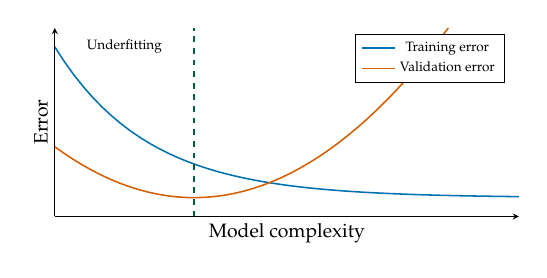
\begin{tikzpicture}[scale=0.7]
    \begin{axis}[
        xlabel={Model complexity}, ylabel={Error},
        xmin=0, xmax=10, ymin=0, ymax=5,
        width=10cm, height=5cm,
        axis lines=left, ticks=none,
        legend pos=north east,
        legend style={font=\scriptsize}
    ]
    \addplot[thick, blue, domain=0:10, samples=50] {4*exp(-0.5*x) + 0.5};
    \addlegendentry{Training error}
    \addplot[thick, red, domain=0:10, samples=50] {0.5 + 0.15*(x-3)^2};
    \addlegendentry{Validation error}
    \draw[dashed, green!60!black, thick] (axis cs:3, 0) -- (axis cs:3, 5);
    \node[green!60!black, font=\scriptsize, above] at (axis cs:3, 5) {optimal};
    \node[font=\scriptsize] at (axis cs:1.5, 4.5) {Underfitting};
    \node[font=\scriptsize] at (axis cs:8, 4.5) {Overfitting};
    \end{axis}
\end{tikzpicture}
\end{center}

\vspace{-4pt}
\textbf{Regularization:} techniques that reduce overfitting by \textbf{constraining} the model.

\vspace{4pt}
\textbf{Today we cover:} L2, L1, dropout, early stopping, data augmentation.
\end{frame}



\begin{frame}
\frametitle{Dropout}

\begin{tikzpicture}
\node [mybox] (box){%
    \begin{minipage}{0.93\textwidth}
    \vspace{-4pt}
    During training, randomly set a fraction $p$ of neurons to zero at each forward pass:
    \[
        \vh_{\text{drop}} = \vh \odot \vm, \qquad m_i \sim \text{Bernoulli}(1-p) \text{ independently}
    \]
    \end{minipage}
};
\node[fancytitle, right=10pt] at (box.north west) {Dropout (Srivastava et al., 2014)};
\end{tikzpicture}

\vspace{6pt}
\textbf{At inference time:} use all neurons, but \textbf{scale} by $(1-p)$ to match expected output during training.

\vspace{6pt}
\textbf{Why dropout works:}
\begin{wideitemize}
    \item \textbf{Prevents co-adaptation}: neurons can't rely on specific others.
    \item \textbf{Ensemble interpretation}: each forward pass uses a different sub-network.
    \item \textbf{Implicit regularization}: similar effect to L2.
\end{wideitemize}

\vspace{6pt}
\textbf{Typical values:} $p = 0.2$ for input layer, $p = 0.5$ for hidden layers.
\end{frame}

\begin{frame}
\frametitle{Dropout: Visual Illustration}

\begin{center}
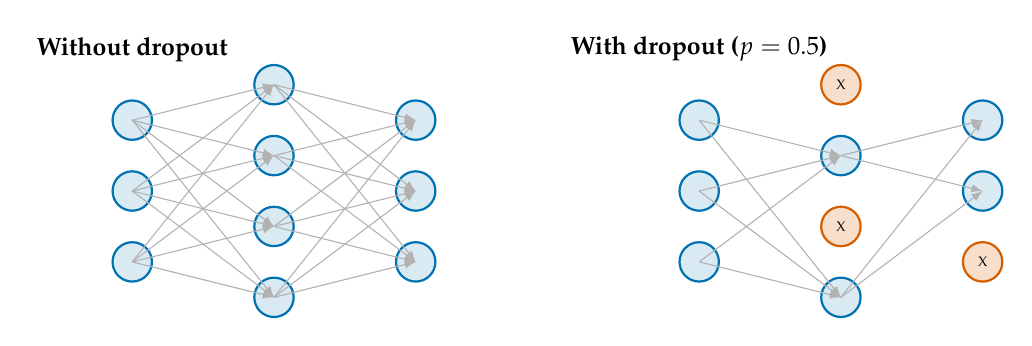
\begin{tikzpicture}[
    neuron/.style={circle, draw, thick, minimum size=0.5cm, font=\tiny},
    >=latex, scale=0.9
]
    % --- Without dropout ---
    \node[font=\small\bfseries] at (0, 3.5) {Without dropout};
    \foreach \y in {0.5, 1.5, 2.5} {
        \node[neuron, draw=blue, fill=blue!15] at (0, \y) {};
    }
    \foreach \y in {0, 1, 2, 3} {
        \node[neuron, draw=blue, fill=blue!15] at (2, \y) {};
    }
    \foreach \y in {0.5, 1.5, 2.5} {
        \node[neuron, draw=blue, fill=blue!15] at (4, \y) {};
    }
    \foreach \yi in {0.5, 1.5, 2.5} {
        \foreach \yj in {0, 1, 2, 3} {
            \draw[->, thin, gray!60] (0, \yi) -- (2, \yj);
        }
    }
    \foreach \yi in {0, 1, 2, 3} {
        \foreach \yj in {0.5, 1.5, 2.5} {
            \draw[->, thin, gray!60] (2, \yi) -- (4, \yj);
        }
    }

    % --- With dropout ---
    \node[font=\small\bfseries] at (8, 3.5) {With dropout ($p=0.5$)};
    \foreach \y in {0.5, 1.5, 2.5} {
        \node[neuron, draw=blue, fill=blue!15] at (8, \y) {};
    }
    \node[neuron, draw=blue, fill=blue!15] at (10, 0) {};
    \node[neuron, draw=red, fill=red!20] at (10, 1) {X};
    \node[neuron, draw=blue, fill=blue!15] at (10, 2) {};
    \node[neuron, draw=red, fill=red!20] at (10, 3) {X};
    \node[neuron, draw=red, fill=red!20] at (12, 0.5) {X};
    \node[neuron, draw=blue, fill=blue!15] at (12, 1.5) {};
    \node[neuron, draw=blue, fill=blue!15] at (12, 2.5) {};

    \foreach \yi in {0.5, 1.5, 2.5} {
        \foreach \yj in {0, 2} {
            \draw[->, thin, gray!60] (8, \yi) -- (10, \yj);
        }
    }
    \foreach \yi in {0, 2} {
        \foreach \yj in {1.5, 2.5} {
            \draw[->, thin, gray!60] (10, \yi) -- (12, \yj);
        }
    }
\end{tikzpicture}
\end{center}

\vspace{8pt}
\textbf{At each training step}, a different random subset of neurons is active.
\end{frame}

\begin{frame}
\frametitle{Early Stopping and Data Augmentation}

\textbf{Early stopping:} monitor validation loss and stop when it stops improving.

\begin{center}
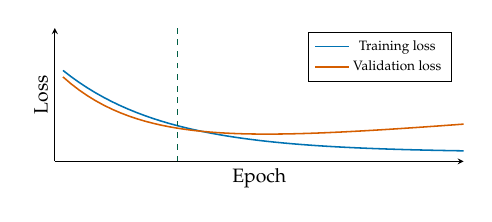
\begin{tikzpicture}[scale=0.7]
    \begin{axis}[
        xlabel={Epoch}, ylabel={Loss},
        xmin=0, xmax=50, ymin=0, ymax=3,
        width=9cm, height=4cm,
        axis lines=left, ticks=none,
        legend pos=north east,
        legend style={font=\scriptsize}
    ]
    \addplot[thick, blue, domain=1:50, samples=50] {2*exp(-0.08*x) + 0.2};
    \addlegendentry{Training loss}
    \addplot[thick, red, domain=1:50, samples=50] {2*exp(-0.1*x) + 0.3 + 0.015*(x - 15)};
    \addlegendentry{Validation loss}
    \draw[dashed, green!60!black, thick] (axis cs:15, 0) -- (axis cs:15, 3);
    \node[green!60!black, font=\scriptsize, above] at (axis cs:15, 3) {stop here};
    \end{axis}
\end{tikzpicture}
\end{center}

\vspace{-4pt}
\textbf{Data augmentation:} create ``new'' training data via transformations.
\begin{itemize}
    \item \textbf{Images:} rotation, flipping, cropping, color jittering.
    \item \textbf{Text:} synonym replacement, back-translation.
    \item \textbf{Time series:} jittering, time warping.
    \item \textbf{Effect:} teach the model \textbf{invariances}.
\end{itemize}
\end{frame}


% ============================================================
\section{Batch Normalization}
% ============================================================

\begin{transitionframe}
\begin{center}
{\Huge \textbf{Batch Normalization}}
\end{center}
\end{transitionframe}

\begin{frame}
\frametitle{The Internal Covariate Shift Problem}

In a deep network, the distribution of activations at each layer \textbf{changes} during training (as earlier layers' weights change).

\vspace{6pt}
\textbf{Consequences:}
\begin{wideitemize}
    \item Each layer must constantly adapt to its input distribution.
    \item Training is slower.
    \item Requires careful initialization and small learning rates.
\end{wideitemize}

\vspace{8pt}
\textbf{Idea (Ioffe \& Szegedy, 2015):} \textcolor{red}{normalize activations} at each layer to have mean 0 and variance 1.

\vspace{6pt}
\textbf{But naive normalization destroys information.} The solution: normalize, then learn scale and shift.
\end{frame}

\begin{frame}
\frametitle{Batch Normalization: The Algorithm}

For a mini-batch $\mathcal{B} = \{x_1, \ldots, x_B\}$:

\vspace{4pt}
\textbf{Step 1 -- Compute batch statistics:}
\[
    \mu_{\mathcal{B}} = \frac{1}{B}\sum_{i=1}^{B} x_i \qquad \sigma_{\mathcal{B}}^2 = \frac{1}{B}\sum_{i=1}^{B} (x_i - \mu_{\mathcal{B}})^2
\]

\textbf{Step 2 -- Normalize:} \quad $\hat{x}_i = \dfrac{x_i - \mu_{\mathcal{B}}}{\sqrt{\sigma_{\mathcal{B}}^2 + \epsilon}}$

\vspace{6pt}
\textbf{Step 3 -- Scale and shift (learnable):} \quad $y_i = \gamma \hat{x}_i + \beta$

\vspace{4pt}
where $\gamma, \beta$ are \textbf{learned parameters} (via backprop).

\vspace{6pt}
\textcolor{red}{\textbf{Key insight:}} if the network learns $\gamma = \sigma_{\mathcal{B}}, \beta = \mu_{\mathcal{B}}$, BN is identity $\Rightarrow$ no loss of expressiveness.
\end{frame}

\begin{frame}
\frametitle{Batch Norm: Training vs Inference}

\textbf{At training time:} use \textbf{batch statistics} $\mu_{\mathcal{B}}, \sigma_{\mathcal{B}}^2$.

\vspace{6pt}
\textbf{At inference time:} batches may have size 1, so batch statistics are unreliable.

\textbf{Solution:} maintain \textbf{running averages} during training:
\begin{align*}
    \mu_{\text{run}} &\leftarrow (1 - m)\mu_{\text{run}} + m \mu_{\mathcal{B}} \\
    \sigma_{\text{run}}^2 &\leftarrow (1 - m)\sigma_{\text{run}}^2 + m \sigma_{\mathcal{B}}^2
\end{align*}

At inference, use $\mu_{\text{run}}, \sigma_{\text{run}}^2$.

\vspace{6pt}
\textbf{Benefits of BN:}
\begin{itemize}
    \item \textcolor{green}{Faster training} (allows higher LR).
    \item \textcolor{green}{Smoother loss landscape} (shown empirically).
    \item \textcolor{green}{Implicit regularization} (batch noise acts as regularization).
    \item \textcolor{green}{Less sensitive to initialization}.
\end{itemize}

\vspace{4pt}
\textbf{Variants:} Layer Norm (Transformers), Group Norm, Instance Norm.
\end{frame}


% ============================================================
\section{Universal Approximation Theorem}
% ============================================================

\begin{transitionframe}
\begin{center}
{\Huge \textbf{Universal Approximation Theorem}}
\end{center}
\end{transitionframe}

\begin{frame}
\frametitle{The Universal Approximation Theorem}

\begin{tikzpicture}
\node [mybox] (box){%
    \begin{minipage}{0.93\textwidth}
    \vspace{-4pt}
    Let $\sigma$ be a non-constant, bounded, monotonically increasing continuous function. Then for any continuous function $f: [0,1]^d \to \R$ and any $\epsilon > 0$, there exist $N \in \mathbb{N}$, $\{w_i\}, \{b_i\}, \{v_i\}$ such that:
    \[
        \left| f(\vx) - \sum_{i=1}^{N} v_i \, \sigma(\vw_i^\top \vx + b_i) \right| < \epsilon \quad \forall \vx \in [0,1]^d
    \]

    \textbf{In words:} a neural network with \textbf{one hidden layer} and \textbf{enough neurons} can approximate any continuous function to arbitrary precision.
    \end{minipage}
};
\node[fancytitle, right=10pt] at (box.north west) {Cybenko (1989), Hornik (1991)};
\end{tikzpicture}

\vspace{6pt}
\textbf{Extensions:}
\begin{itemize}
    \item Works for sigmoid, tanh, ReLU (with adjustments).
    \item Also holds for any Lebesgue-measurable function.
\end{itemize}
\end{frame}

\begin{frame}
\frametitle{UAT: Proof Sketch (Geometric Intuition)}

\textbf{Goal:} approximate any function $f(x)$ with a sum of sigmoids.

\vspace{4pt}
\textbf{Step 1:} A single sigmoid can approximate a \textbf{step function} (with large $w$):
\[
    \sigma(wx + b) \approx \begin{cases} 1 & x > -b/w \\ 0 & x < -b/w \end{cases} \quad \text{for large } w
\]

\textbf{Step 2:} Two sigmoids with opposite weights create a \textbf{bump} function:
\[
    \sigma(w(x - a)) - \sigma(w(x - a - h)) \approx \text{bump on } [a, a+h]
\]

\textbf{Step 3:} Sum many bumps $\to$ approximate any continuous function (like Riemann integration!).

\vspace{8pt}
\textbf{Formal argument:} uses the Hahn-Banach theorem + Riesz representation theorem.

\vspace{6pt}
\begin{center}
\textcolor{red}{\textbf{Key insight:} sigmoids form a dense subset of continuous functions on compact sets.}
\end{center}
\end{frame}

\begin{frame}
\frametitle{But Why Depth Then?}

\textbf{UAT says:} one hidden layer is enough. But in practice, we use \textbf{deep} networks.

\vspace{6pt}
\textbf{Problem with shallow networks:} the required width can grow \textbf{exponentially} with complexity.

\vspace{6pt}
\begin{tikzpicture}
\node [mybox] (box){%
    \begin{minipage}{0.93\textwidth}
    \vspace{-4pt}
    \textbf{Depth-width tradeoff (Telgarsky, 2016):}

    There exist functions that can be represented by a network of depth $L$ with $O(L)$ neurons, but require $\Omega(2^L)$ neurons in a shallow network.
    \end{minipage}
};
\node[fancytitle, right=10pt] at (box.north west) {Theorem};
\end{tikzpicture}

\vspace{8pt}
\textbf{Why deep works:}
\begin{wideitemize}
    \item \textbf{Hierarchical features}: edges $\to$ parts $\to$ objects.
    \item \textbf{Compositional structure}: natural data is compositional.
    \item \textbf{Exponential efficiency}: depth is \textbf{exponentially more parameter-efficient}.
\end{wideitemize}
\end{frame}



% ============================================================
\section{GPUs and Parallel Computing}
% ============================================================

\begin{transitionframe}
\begin{center}
{\Huge \textbf{GPUs and Parallel Computing}}
\end{center}
\end{transitionframe}

\begin{frame}
\frametitle{CPU vs GPU Architecture}

\begin{columns}[T]
\begin{column}{0.48\textwidth}
\centering
\textcolor{blue}{\textbf{CPU}}

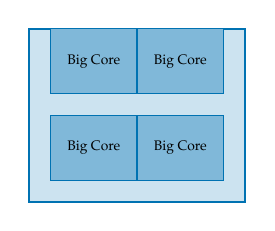
\begin{tikzpicture}[scale=0.55]
    \draw[fill=blue!20, draw=blue, thick] (0,0) rectangle (5, 4);
    \foreach \x in {0.5, 2.5} {
        \foreach \y in {0.5, 2.5} {
            \draw[fill=blue!50, draw=blue] (\x, \y) rectangle (\x+2, \y+1.5);
        }
    }
    \node[font=\tiny] at (1.5, 1.25) {Big Core};
    \node[font=\tiny] at (3.5, 1.25) {Big Core};
    \node[font=\tiny] at (1.5, 3.25) {Big Core};
    \node[font=\tiny] at (3.5, 3.25) {Big Core};
\end{tikzpicture}

\begin{itemize}
    \item Few powerful cores (4--64).
    \item Optimized for \textbf{sequential} execution.
    \item Great for branching logic.
\end{itemize}
\end{column}

\begin{column}{0.48\textwidth}
\centering
\textcolor{red}{\textbf{GPU}}

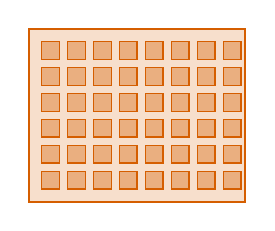
\begin{tikzpicture}[scale=0.55]
    \draw[fill=red!20, draw=red, thick] (0,0) rectangle (5, 4);
    \foreach \x in {0.3, 0.9, 1.5, 2.1, 2.7, 3.3, 3.9, 4.5} {
        \foreach \y in {0.3, 0.9, 1.5, 2.1, 2.7, 3.3} {
            \draw[fill=red!50, draw=red] (\x, \y) rectangle (\x+0.4, \y+0.4);
        }
    }
\end{tikzpicture}

\begin{itemize}
    \item Thousands of simple cores.
    \item Optimized for \textbf{parallel} execution.
    \item Great for matrix operations.
\end{itemize}
\end{column}
\end{columns}

\vspace{6pt}
\textbf{Why GPUs dominate DL:} neural networks are mostly \textbf{matrix multiplications}, which are embarrassingly parallel. A $1000 \times 1000$ matmul: CPU = seconds, GPU = milliseconds.
\end{frame}

\begin{frame}[fragile]
\frametitle{Using GPUs in PyTorch}

\begin{lstlisting}
import torch

# Check if GPU is available
device = torch.device('cuda' if torch.cuda.is_available() else 'cpu')
print(f"Using device: {device}")

# Move tensors to GPU
x = torch.randn(1000, 1000).to(device)
y = torch.randn(1000, 1000).to(device)
z = x @ y                    # Matmul on GPU

# Move model to GPU
model = MyNeuralNetwork().to(device)

# Move batches to GPU during training
for X_batch, y_batch in loader:
    X_batch, y_batch = X_batch.to(device), y_batch.to(device)
    y_pred = model(X_batch)
    loss = criterion(y_pred, y_batch)
\end{lstlisting}

\textbf{Rule:} both model and data must be on the \textbf{same device}.
\end{frame}

\begin{frame}
\frametitle{Parallelism Strategies}

\textbf{Data parallelism} (most common):
\begin{itemize}
    \item Replicate model across multiple GPUs.
    \item Split batch across GPUs.
    \item Average gradients after each step.
    \item PyTorch: \texttt{nn.DataParallel}, \texttt{nn.DistributedDataParallel}.
\end{itemize}

\vspace{6pt}
\textbf{Model parallelism} (for huge models):
\begin{itemize}
    \item Split model across multiple GPUs.
    \item Used for LLMs that don't fit in one GPU.
\end{itemize}

\vspace{6pt}
\textbf{Mixed precision training (AMP):}
\begin{itemize}
    \item Use float16 instead of float32 where possible.
    \item \textbf{2x faster} on modern GPUs (tensor cores).
    \item PyTorch: \texttt{torch.cuda.amp.autocast}.
\end{itemize}

\vspace{6pt}
\textbf{For this course:} Google Colab GPUs are enough (T4, A100).
\end{frame}


% ============================================================
\section{Practical Recipe and Summary}
% ============================================================

\begin{transitionframe}
\begin{center}
{\Huge \textbf{Practical Recipe \& Summary}}
\end{center}
\end{transitionframe}

\begin{frame}
\frametitle{The Deep Learning Training Recipe}

A checklist for training deep networks:

\begin{enumerate}
    \item \textbf{Normalize your inputs} (mean 0, std 1 per feature).
    \item \textbf{Initialize weights properly:} He (ReLU) or Xavier (sigmoid/tanh).
    \item \textbf{Choose architecture:} start simple, add complexity as needed.
    \item \textbf{Add batch normalization} to hidden layers.
    \item \textbf{Pick optimizer:} start with \textbf{Adam} (LR = $10^{-3}$).
    \item \textbf{Add regularization:} dropout (0.2-0.5) or weight decay ($10^{-4}$).
    \item \textbf{Monitor train and validation loss} at each epoch.
    \item \textbf{Use early stopping} based on validation loss.
    \item \textbf{Scale up}: batch size, depth, width, data augmentation.
\end{enumerate}

\vspace{6pt}
\textbf{Debugging tips:}
\begin{itemize}
    \item If loss is NaN: LR too high or bad init.
    \item If loss doesn't decrease: check gradients, try different optimizer.
    \item If overfitting: more regularization, more data, smaller model.
\end{itemize}
\end{frame}

\begin{frame}
\frametitle{Summary}

\begin{enumerate}
    \item \textbf{Optimizers:} Adam combines momentum + adaptive LR + bias correction. Default choice.

    \item \textbf{Initialization:} Xavier for sigmoid/tanh, He for ReLU.

    \item \textbf{Regularization:} L2 shrinks weights, L1 induces sparsity, dropout breaks co-adaptation.

    \item \textbf{Batch Normalization:} normalize activations per batch, with learnable $\gamma, \beta$.

    \item \textbf{UAT:} one hidden layer is enough \textit{in theory}, but depth is \textbf{exponentially more efficient} for compositional functions.

    \item \textbf{GPUs:} parallelism enables training of large models. Use PyTorch \texttt{.to(device)}.
\end{enumerate}
\end{frame}






\tikzset{
        every picture/.style={remember picture,baseline},
        every node/.style={anchor=base,align=center,outer sep=1.5pt},
        every path/.style={thick},
        }
\tikzstyle{every picture}+=[remember picture]
\tikzstyle{mybox} =[draw=black, very thick, rectangle, inner sep=10pt, inner ysep=20pt]
\tikzstyle{fancytitle} =[draw=black,fill=red, text=white]




% ============================================================
\section{Recap and Motivation}
% ============================================================

\begin{transitionframe}
\begin{center}
{\Huge \textbf{Recap \& Motivation}}\\[10pt]
{\large Why do we need CNNs?}
\end{center}
\end{transitionframe}


\begin{frame}
\frametitle{The Problem with Fully-Connected Networks for Images}

Consider a $100 \times 100$ grayscale image flattened to a vector of $10{,}000$ pixels.

\vspace{4pt}
A fully-connected layer with $H$ hidden units has $10{,}000 \times H$ weights:

\renewcommand{\arraystretch}{1.3}
\begin{center}
{\small
\begin{tabular}{cc}
\toprule
\textbf{Hidden units} $H$ & \textbf{Weights} (input layer only) \\
\midrule
1 & 10,000 \\
100 & 1,000,000 \\
1,000 & 10,000,000 \\
10,000 & 100,000,000 \\
\textcolor{red}{100,000} & \textcolor{red}{1,000,000,000 (\textbf{1 billion!})} \\
\bottomrule
\end{tabular}
}
\end{center}

\vspace{6pt}
\textbf{And this is just one layer of a small grayscale image.}

\vspace{4pt}
Real images: $224 \times 224 \times 3 = 150{,}528$ inputs. Real datasets (ImageNet): 1.2M images.

\vspace{4pt}
\textcolor{red}{Parameter explosion + insufficient data $\Rightarrow$ severe overfitting.}
\end{frame}

\begin{frame}
\frametitle{Two Components to Solve Any Task}

\begin{center}
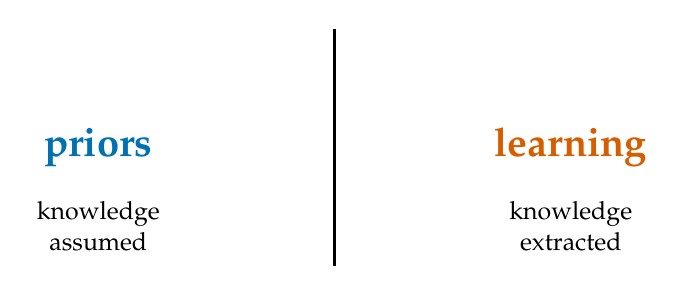
\begin{tikzpicture}[scale=1.0]
    \draw[very thick] (0, 0) -- (0, 3);
    \node[font=\Large\bfseries, blue] at (-3, 1.5) {priors};
    \node[font=\Large\bfseries, red] at (3, 1.5) {learning};

    \node[font=\small, align=center] at (-3, 0.5) {knowledge\\assumed};
    \node[font=\small, align=center] at (3, 0.5) {knowledge\\extracted};
\end{tikzpicture}
\end{center}

\vspace{8pt}
\textbf{Strong priors, minimal learning} $\to$ fast/easy, but \textbf{rigid}.

\vspace{4pt}
\textbf{Weak priors, much learning} $\to$ flexible, but \textbf{slow/data-hungry}.

\vspace{8pt}
\begin{center}
\textcolor{red}{For images, we need to add the right \textbf{inductive biases} (priors) to make learning tractable.}
\end{center}
\end{frame}


% ============================================================
\section{Inductive Biases for Images}
% ============================================================

\begin{transitionframe}
\begin{center}
{\Huge \textbf{Inductive Biases for Images}}
\end{center}
\end{transitionframe}

\begin{frame}
\frametitle{Locality: Nearby Pixels Share Patterns}

\begin{columns}[T]
\begin{column}{0.5\textwidth}
\textbf{Observation:} structure in images is \textbf{local}.

\vspace{6pt}
\begin{itemize}
    \item Nearby \textbf{pixels} are correlated (sky, grass, skin all show smooth color gradients).
    \item Nearby \textbf{patches} form features (edges, textures).
    \item Nearby \textbf{regions} form parts (eyes, mouths, wheels).
\end{itemize}

\vspace{8pt}
\textbf{Inductive bias:} a feature at one location should depend \textbf{only on its local neighborhood}, not on distant pixels.
\end{column}

\begin{column}{0.45\textwidth}
\begin{center}
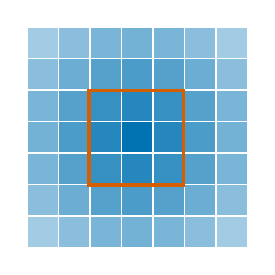
\begin{tikzpicture}[scale=0.4]
    \foreach \i in {0,1,2,3,4,5,6} {
        \foreach \j in {0,1,2,3,4,5,6} {
            \pgfmathsetmacro{\dist}{sqrt((\i-3)^2 + (\j-3)^2)}
            \pgfmathsetmacro{\intensity}{max(0, 100 - 15*\dist)}
            \fill[blue!\intensity] (\i, \j) rectangle ++(0.95, 0.95);
        }
    }
    \draw[red, very thick] (1.95, 1.95) rectangle (4.95, 4.95);
\end{tikzpicture}
\end{center}

{\small \centering A $3 \times 3$ neighborhood (red box) captures the local structure.}
\end{column}
\end{columns}
\end{frame}

\begin{frame}
\frametitle{Translation Invariance: Position-Independent Features}

\textbf{Observation:} the identity of an object does not depend on its absolute position.

\vspace{6pt}
\begin{center}
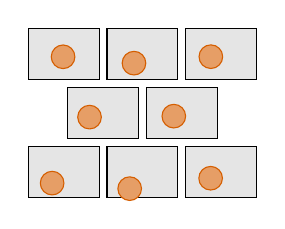
\begin{tikzpicture}[scale=0.5]
    \foreach \i/\j in {0/0, 2/0, 4/0, 1/1.5, 3/1.5, 0/3, 2/3, 4/3} {
        \draw[fill=gray!20, draw=black] (\i, \j) rectangle ++(1.8, 1.3);
        \draw[fill=red!60, draw=red] (\i+0.6+0.3*rand, \j+0.4+0.2*rand) circle (0.3);
    }
\end{tikzpicture}
\end{center}

\vspace{6pt}
\textbf{Example:} a cat is a cat whether it appears in the top-left or bottom-right of the image.

\vspace{8pt}
\textbf{Inductive bias:} the same \textbf{feature detector} should be applied at every spatial location $\Rightarrow$ \textcolor{red}{weight sharing across positions}.
\end{frame}

\begin{frame}
\frametitle{From Inductive Biases to CNNs}

\textbf{Two key inductive biases for images:}

\vspace{6pt}
\begin{center}
\renewcommand{\arraystretch}{1.4}
\begin{tabular}{ll}
\toprule
\textbf{Property} & \textbf{Architectural implementation} \\
\midrule
\textcolor{blue}{\textbf{Locality}} & Each output depends on a \textbf{small spatial region} of the input \\
\textcolor{red}{\textbf{Translation invariance}} & The \textbf{same filter weights} are reused at every location \\
\bottomrule
\end{tabular}
\end{center}

\vspace{10pt}
\begin{center}
\fbox{\textbf{Together: Convolutional Neural Networks (CNNs)}}
\end{center}

\vspace{8pt}
\textbf{Consequences:}
\begin{itemize}
    \item Number of parameters becomes \textbf{independent of input size}.
    \item The model generalizes much better with limited data.
    \item Computationally efficient (parallelizable on GPUs).
\end{itemize}
\end{frame}


% ============================================================
\section{The Convolution Operation}
% ============================================================

\begin{transitionframe}
\begin{center}
{\Huge \textbf{The Convolution Operation}}
\end{center}
\end{transitionframe}

\begin{frame}
\frametitle{1D Convolution: Mathematical Definition}

\begin{tikzpicture}
\node [mybox] (box){%
    \begin{minipage}{0.93\textwidth}
    \vspace{-6pt}
    Given input $\vx \in \R^n$ and kernel $\vK \in \R^k$, the (cross-)convolution is:
    \[
        (\vx * \vK)[i] = \sum_{j=0}^{k-1} \vx[i + j] \cdot \vK[j]
    \]
    \vspace{-8pt}
    \end{minipage}
};
\node[fancytitle, right=10pt] at (box.north west) {1D Convolution};
\end{tikzpicture}

\vspace{2pt}
\textbf{Note:} in DL, ``convolution'' usually means cross-correlation (no kernel flipping).

\vspace{2pt}
\textbf{Intuition:} slide the kernel across the input, computing dot products at each position.

\vspace{2pt}
\textbf{Example:} input $\vx = (1, 2, 3, 4, 5)$, kernel $\vK = (1, 0, -1)$:
\begin{align*}
    \text{output}[0] &= 1{\cdot}1 + 2{\cdot}0 + 3{\cdot}(-1) = -2 \\
    \text{output}[1] &= 2{\cdot}1 + 3{\cdot}0 + 4{\cdot}(-1) = -2 \\
    \text{output}[2] &= 3{\cdot}1 + 4{\cdot}0 + 5{\cdot}(-1) = -2
\end{align*}
\end{frame}

\begin{frame}
\frametitle{2D Convolution: Numerical Example}

\textbf{Input image} $5 \times 5$ \quad and \quad \textbf{kernel} $3 \times 3$:

\begin{center}
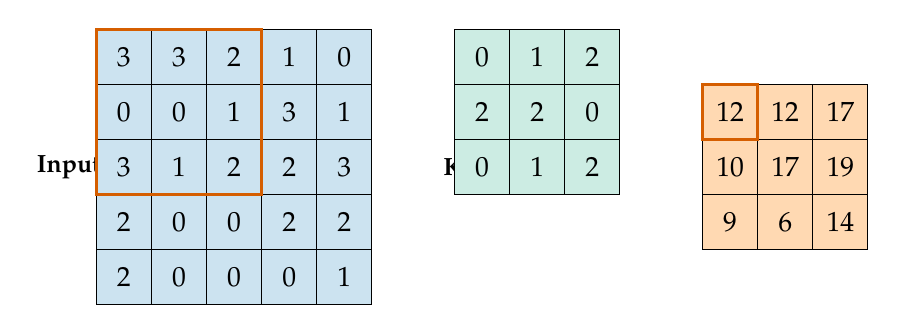
\begin{tikzpicture}[scale=0.7]
    % Input image
    \node at (-0.5, 2.5) {\small \textbf{Input}};
    \foreach \i/\j/\v in {0/0/3, 1/0/3, 2/0/2, 3/0/1, 4/0/0,
                          0/1/0, 1/1/0, 2/1/1, 3/1/3, 4/1/1,
                          0/2/3, 1/2/1, 2/2/2, 3/2/2, 4/2/3,
                          0/3/2, 1/3/0, 2/3/0, 3/3/2, 4/3/2,
                          0/4/2, 1/4/0, 2/4/0, 3/4/0, 4/4/1} {
        \draw[fill=blue!20] (\i, 4-\j) rectangle ++(1, 1);
        \node at (\i+0.5, 4-\j+0.5) {\v};
    }
    % Highlighted region
    \draw[red, very thick] (0, 2) rectangle (3, 5);

    % Kernel
    \node at (7, 2.5) {\small \textbf{Kernel}};
    \foreach \i/\j/\v in {0/0/0, 1/0/1, 2/0/2,
                          0/1/2, 1/1/2, 2/1/0,
                          0/2/0, 1/2/1, 2/2/2} {
        \draw[fill=green!20] (6.5+\i, 4-\j) rectangle ++(1, 1);
        \node at (7+\i, 4-\j+0.5) {\v};
    }

    % Output
    \node at (12, 2.5) {\small \textbf{Output}};
    \foreach \i/\j/\v in {0/0/12, 1/0/12, 2/0/17,
                          0/1/10, 1/1/17, 2/1/19,
                          0/2/9, 1/2/6, 2/2/14} {
        \draw[fill=orange!30] (11+\i, 3-\j) rectangle ++(1, 1);
        \node at (11.5+\i, 3-\j+0.5) {\v};
    }
    \draw[red, very thick] (11, 3) rectangle (12, 4);
\end{tikzpicture}
\end{center}

\vspace{4pt}
\textbf{Output[0,0]} (red region) $= 3 \cdot 0 + 3 \cdot 1 + 2 \cdot 2 + 0 \cdot 2 + 0 \cdot 2 + 1 \cdot 0 + 3 \cdot 0 + 1 \cdot 1 + 2 \cdot 2 = \textcolor{red}{12}$

\vspace{4pt}
Slide the kernel one position $\to$ compute next output, etc.
\end{frame}

\begin{frame}
\frametitle{Stride and Padding}

\textbf{Stride $S$:} how many pixels the kernel moves per step. \quad \textbf{Padding $P$:} zeros around the border.

\vspace{4pt}
\begin{columns}[T]
\begin{column}{0.48\textwidth}
\centering
\textcolor{blue}{\textbf{Stride = 1, no padding}}\\
{\small Output smaller than input}

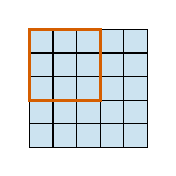
\begin{tikzpicture}[scale=0.3]
    \foreach \i in {0,1,2,3,4} {
        \foreach \j in {0,1,2,3,4} {
            \draw[fill=blue!20] (\i, \j) rectangle ++(1, 1);
        }
    }
    \draw[red, very thick] (0, 2) rectangle (3, 5);
\end{tikzpicture}
\end{column}

\begin{column}{0.48\textwidth}
\centering
\textcolor{red}{\textbf{Stride = 1, padding = 1 (``same'')}}\\
{\small Output same size as input}

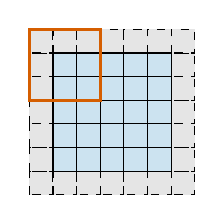
\begin{tikzpicture}[scale=0.3]
    \foreach \i in {-1,0,1,2,3,4,5} {
        \foreach \j in {-1,0,1,2,3,4,5} {
            \draw[fill=gray!20, dashed] (\i, \j) rectangle ++(1, 1);
        }
    }
    \foreach \i in {0,1,2,3,4} {
        \foreach \j in {0,1,2,3,4} {
            \draw[fill=blue!20] (\i, \j) rectangle ++(1, 1);
        }
    }
    \draw[red, very thick] (-1, 3) rectangle (2, 6);
\end{tikzpicture}
\end{column}
\end{columns}

\vspace{4pt}
\begin{tikzpicture}
\node [mybox] (box){%
    \begin{minipage}{0.93\textwidth}
    \vspace{-8pt}
    \[
        W_{\text{out}} = \left\lfloor \frac{W_{\text{in}} + 2P - F}{S} \right\rfloor + 1
    \]
    \vspace{-6pt}\\
    {\footnotesize $W_{\text{in}}$: input width \quad $F$: filter (kernel) size \quad $P$: padding \quad $S$: stride}
    \end{minipage}
};
\node[fancytitle, right=10pt] at (box.north west) {Output Size Formula};
\end{tikzpicture}
\end{frame}

\begin{frame}
\frametitle{Output Size: Worked Examples}

\textbf{Formula:} \quad $W_{\text{out}} = \lfloor (W_{\text{in}} + 2P - F)/S \rfloor + 1$

\vspace{8pt}
\renewcommand{\arraystretch}{1.4}
\begin{center}
{\small
\begin{tabular}{ccccc|c}
\toprule
\textbf{$W_{\text{in}}$} & \textbf{Filter $F$} & \textbf{Padding $P$} & \textbf{Stride $S$} & \textbf{Computation} & \textbf{$W_{\text{out}}$} \\
\midrule
$28$ & $3$ & $0$ & $1$ & $\lfloor (28 + 0 - 3)/1 \rfloor + 1$ & $26$ \\
$28$ & $3$ & $1$ & $1$ & $\lfloor (28 + 2 - 3)/1 \rfloor + 1$ & $\textcolor{red}{28}$ \\
$28$ & $5$ & $2$ & $1$ & $\lfloor (28 + 4 - 5)/1 \rfloor + 1$ & $\textcolor{red}{28}$ \\
$224$ & $3$ & $1$ & $2$ & $\lfloor (224 + 2 - 3)/2 \rfloor + 1$ & $\textcolor{red}{112}$ \\
$224$ & $7$ & $3$ & $2$ & $\lfloor (224 + 6 - 7)/2 \rfloor + 1$ & $\textcolor{red}{112}$ \\
\bottomrule
\end{tabular}
}
\end{center}

\vspace{8pt}
\textbf{Common patterns:}
\begin{itemize}
    \item \textbf{``Same'' convolution} ($P = (F-1)/2$, $S=1$): preserves size. Useful for stacking layers.
    \item \textbf{Strided convolution} ($S = 2$): halves spatial size. Used for downsampling.
\end{itemize}
\end{frame}

\begin{frame}
\frametitle{Filters as Feature Detectors}

\textbf{Different kernels detect different features:}

\vspace{6pt}
\begin{columns}[T]
\begin{column}{0.32\textwidth}
\centering
\textcolor{blue}{\textbf{Sobel (vertical edges)}}

\[
    \begin{pmatrix} -1 & 0 & 1 \\ -2 & 0 & 2 \\ -1 & 0 & 1 \end{pmatrix}
\]

\vspace{2pt}
{\scriptsize Detects vertical changes in intensity.}
\end{column}

\begin{column}{0.32\textwidth}
\centering
\textcolor{blue}{\textbf{Gaussian (blur)}}

\[
    \frac{1}{16}\begin{pmatrix} 1 & 2 & 1 \\ 2 & 4 & 2 \\ 1 & 2 & 1 \end{pmatrix}
\]

\vspace{2pt}
{\scriptsize Smooths the image.}
\end{column}

\begin{column}{0.32\textwidth}
\centering
\textcolor{blue}{\textbf{Sharpen}}

\[
    \begin{pmatrix} 0 & -1 & 0 \\ -1 & 5 & -1 \\ 0 & -1 & 0 \end{pmatrix}
\]

\vspace{2pt}
{\scriptsize Enhances edges.}
\end{column}
\end{columns}

\vspace{12pt}
\textbf{Key insight:} in classical computer vision, these filters were \textbf{hand-designed}.

\vspace{4pt}
\begin{center}
\textcolor{red}{In CNNs, the filters are \textbf{learned} from data via backpropagation.}
\end{center}
\end{frame}


% ============================================================
\section{Convolutional Layers}
% ============================================================

\begin{transitionframe}
\begin{center}
{\Huge \textbf{Convolutional Layers}}
\end{center}
\end{transitionframe}

\begin{frame}
\frametitle{Multiple Input Channels (RGB Images)}

A color image has \textbf{3 channels} (R, G, B). The kernel must also have 3 channels.

\vspace{6pt}
\begin{center}
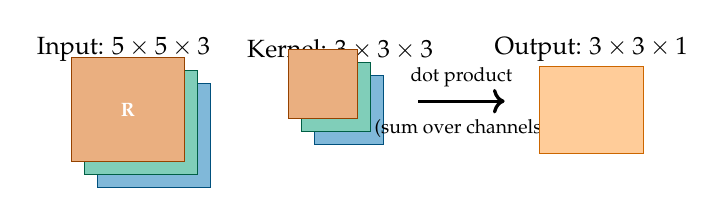
\begin{tikzpicture}[scale=0.55]
    % Input channels (with proper offset and labels)
    \node[font=\small] at (1.2, 5.8) {Input: $5 \times 5 \times 3$};
    \draw[fill=blue!50, draw=blue!70!black] (0.6, 2.6) rectangle (3.2, 5.0);
    \node[white, font=\scriptsize\bfseries] at (1.9, 3.8) {B};
    \draw[fill=green!50, draw=green!60!black] (0.3, 2.9) rectangle (2.9, 5.3);
    \node[white, font=\scriptsize\bfseries] at (1.6, 4.1) {G};
    \draw[fill=red!50, draw=red!70!black] (0, 3.2) rectangle (2.6, 5.6);
    \node[white, font=\scriptsize\bfseries] at (1.3, 4.4) {R};

    % Kernel (well separated)
    \node[font=\small] at (6.2, 5.8) {Kernel: $3 \times 3 \times 3$};
    \draw[fill=blue!50, draw=blue!70!black] (5.6, 3.6) rectangle (7.2, 5.2);
    \draw[fill=green!50, draw=green!60!black] (5.3, 3.9) rectangle (6.9, 5.5);
    \draw[fill=red!50, draw=red!70!black] (5.0, 4.2) rectangle (6.6, 5.8);

    % Arrow with label below to avoid collision
    \draw[->, very thick] (8.0, 4.6) -- (10.0, 4.6);
    \node[above, font=\scriptsize] at (9.0, 4.7) {dot product};
    \node[below, font=\scriptsize] at (9.0, 4.4) {(sum over channels)};

    % Output
    \node[font=\small] at (12.0, 5.8) {Output: $3 \times 3 \times 1$};
    \draw[fill=orange!40, draw=orange!80!black] (10.8, 3.4) rectangle (13.2, 5.4);
\end{tikzpicture}
\end{center}

\vspace{4pt}
\textbf{Math:} for input with $C_{in}$ channels and a $F \times F \times C_{in}$ kernel:
\[
    \text{output}[i, j] = \sum_{c=1}^{C_{in}} \sum_{u=0}^{F-1} \sum_{v=0}^{F-1} \text{input}[i+u, j+v, c] \cdot \text{kernel}[u, v, c] + b
\]

\textcolor{red}{Each filter ``sees'' all input channels but produces a \textbf{single} output channel.}
\end{frame}

\begin{frame}
\frametitle{Multiple Filters $\to$ Multiple Output Channels}

\textbf{One filter} produces one output channel (feature map).

\textbf{Multiple filters} produce multiple output channels.

\vspace{6pt}
\begin{center}
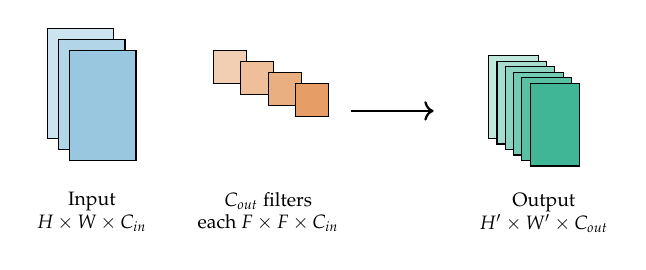
\begin{tikzpicture}[scale=0.7]
    % Input volume
    \draw[fill=blue!20] (0, 0) rectangle (1.2, 2);
    \draw[fill=blue!30] (0.2, -0.2) rectangle (1.4, 1.8);
    \draw[fill=blue!40] (0.4, -0.4) rectangle (1.6, 1.6);
    \node[below] at (0.8, -0.8) {\scriptsize Input};
    \node[below] at (0.8, -1.2) {\scriptsize $H \times W \times C_{in}$};

    % 4 filters
    \foreach \i in {0,1,2,3} {
        \draw[fill=red!\the\numexpr 30+10*\i\relax] (3+0.5*\i, 1-0.2*\i) rectangle ++(0.6, 0.6);
    }
    \node[below] at (4, -0.8) {\scriptsize $C_{out}$ filters};
    \node[below] at (4, -1.2) {\scriptsize each $F \times F \times C_{in}$};

    % Arrow
    \draw[->, thick] (5.5, 0.5) -- (7, 0.5);

    % Output volume (more channels)
    \foreach \i in {0,1,2,3,4,5} {
        \draw[fill=green!\the\numexpr 25+10*\i\relax] (8+0.15*\i, 0-0.1*\i) rectangle ++(0.9, 1.5);
    }
    \node[below] at (9, -0.8) {\scriptsize Output};
    \node[below] at (9, -1.2) {\scriptsize $H' \times W' \times C_{out}$};
\end{tikzpicture}
\end{center}

\vspace{4pt}
\textbf{Total parameters} for one conv layer:
\[
    \underbrace{F \times F \times C_{in} \times C_{out}}_{\text{weights}} + \underbrace{C_{out}}_{\text{biases}}
\]
\end{frame}

\begin{frame}
\frametitle{Parameter Comparison: FC vs Conv}

\textbf{Setting:} input $224 \times 224 \times 3$, output 64 feature maps.

\vspace{6pt}
\renewcommand{\arraystretch}{1.5}
\begin{center}
\begin{tabular}{lll}
\toprule
\textbf{Layer type} & \textbf{Parameter count} & \textbf{Total} \\
\midrule
Fully-connected & $224 \times 224 \times 3 \times 64 = $ & \textcolor{red}{9,633,792} \\
Conv ($3 \times 3$) & $3 \times 3 \times 3 \times 64 + 64 = $ & \textcolor{green}{1,792} \\
Conv ($5 \times 5$) & $5 \times 5 \times 3 \times 64 + 64 = $ & \textcolor{green}{4,864} \\
Conv ($7 \times 7$) & $7 \times 7 \times 3 \times 64 + 64 = $ & \textcolor{green}{9,472} \\
\bottomrule
\end{tabular}
\end{center}

\vspace{8pt}
\begin{center}
\fbox{\textbf{CNN uses $\approx 5{,}000\times$ fewer parameters than FC for the same task.}}
\end{center}

\vspace{6pt}
\textbf{Why?}
\begin{itemize}
    \item \textbf{Locality:} each output uses only a small input region.
    \item \textbf{Weight sharing:} the same kernel is reused at every spatial location.
\end{itemize}
\end{frame}

\begin{frame}
\frametitle{Receptive Field}

\textbf{Definition:} the receptive field of a neuron is the region of the \textbf{input image} that affects its output.

\vspace{4pt}
\begin{center}
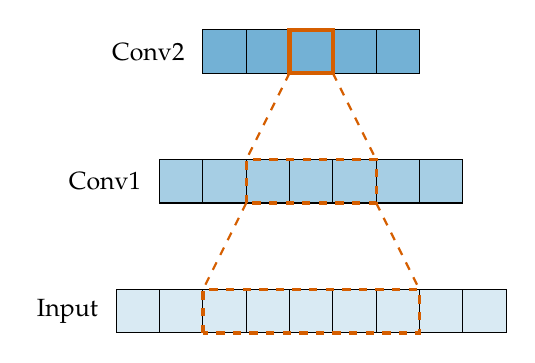
\begin{tikzpicture}[scale=0.55]
    % Layer 0 (input) -- 9 cells
    \foreach \i in {0,...,8} {
        \draw[fill=blue!15, draw=black] (\i, 0) rectangle ++(1, 1);
    }
    \node[left, font=\small] at (-0.2, 0.5) {Input};

    % Layer 1 (Conv1) -- 7 cells, centered
    \foreach \i in {0,...,6} {
        \draw[fill=blue!35, draw=black] (\i+1, 3) rectangle ++(1, 1);
    }
    \node[left, font=\small] at (0.8, 3.5) {Conv1};

    % Layer 2 (Conv2) -- 5 cells, centered
    \foreach \i in {0,...,4} {
        \draw[fill=blue!55, draw=black] (\i+2, 6) rectangle ++(1, 1);
    }
    \node[left, font=\small] at (1.8, 6.5) {Conv2};

    % Highlight target neuron in Conv2 (center)
    \draw[red, very thick, line width=1.5pt] (4, 6) rectangle (5, 7);

    % Receptive field at Conv1 (3 cells: index 3, 4, 5)
    \draw[red, dashed, very thick] (3, 3) rectangle (6, 4);

    % Receptive field at Input (5 cells: index 2, 3, 4, 5, 6)
    \draw[red, dashed, very thick] (2, 0) rectangle (7, 1);

    % Lines from Conv2 down to Conv1 (fan out)
    \draw[red, dashed, thick] (4, 6) -- (3, 4);
    \draw[red, dashed, thick] (5, 6) -- (6, 4);

    % Lines from Conv1 down to Input (fan out)
    \draw[red, dashed, thick] (3, 3) -- (2, 1);
    \draw[red, dashed, thick] (6, 3) -- (7, 1);
\end{tikzpicture}
\end{center}

\vspace{4pt}
\textbf{Each layer uses a $3 \times 3$ kernel} (1D simplification: $1 \times 3$):
\begin{itemize}
    \item Layer 1 neuron sees \textbf{3} input pixels.
    \item Layer 2 neuron sees \textbf{5} input pixels.
    \item Layer $L$ neuron sees \textbf{$2L+1$} input pixels.
\end{itemize}

\textcolor{red}{Receptive field grows linearly with depth $\Rightarrow$ deep CNNs ``see'' the whole image.}
\end{frame}

% ---- Why Receptive Field Matters ----
\begin{frame}
\frametitle{Why Does Receptive Field Matter?}

\textbf{Key principle:} a neuron's output depends \textbf{only} on the pixels inside its receptive field. Anything outside is invisible to it.

\vspace{6pt}
\begin{center}
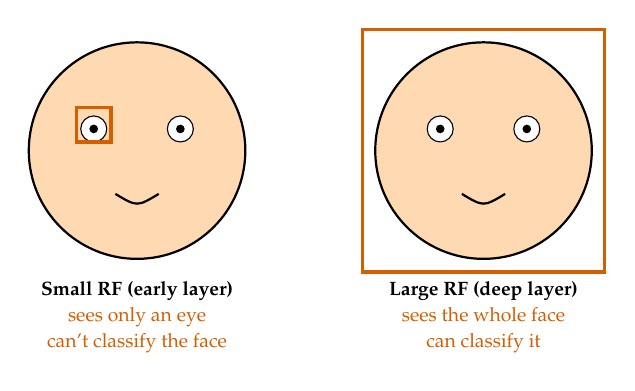
\begin{tikzpicture}[scale=0.55]
    % LEFT: small RF (cannot see whole face)
    \begin{scope}
    % Stylized face
    \draw[fill=orange!30, draw=black, thick] (3, 3) circle (2.5);
    \draw[fill=white, draw=black] (2, 3.5) circle (0.3);
    \draw[fill=white, draw=black] (4, 3.5) circle (0.3);
    \fill (2, 3.5) circle (0.1);
    \fill (4, 3.5) circle (0.1);
    \draw[thick] (2.5, 2) .. controls (3, 1.7) .. (3.5, 2);
    % Small RF box
    \draw[red, very thick] (1.6, 3.2) rectangle (2.4, 4);
    \node[below, font=\scriptsize] at (3, 0.2) {\textbf{Small RF (early layer)}};
    \node[below, font=\scriptsize, text=red] at (3, -0.4) {sees only an eye};
    \node[below, font=\scriptsize, text=red] at (3, -1.0) {can't classify the face};
    \end{scope}

    % RIGHT: large RF (covers whole face)
    \begin{scope}[xshift=8cm]
    \draw[fill=orange!30, draw=black, thick] (3, 3) circle (2.5);
    \draw[fill=white, draw=black] (2, 3.5) circle (0.3);
    \draw[fill=white, draw=black] (4, 3.5) circle (0.3);
    \fill (2, 3.5) circle (0.1);
    \fill (4, 3.5) circle (0.1);
    \draw[thick] (2.5, 2) .. controls (3, 1.7) .. (3.5, 2);
    % Large RF box
    \draw[red, very thick] (0.2, 0.2) rectangle (5.8, 5.8);
    \node[below, font=\scriptsize] at (3, 0.2) {\textbf{Large RF (deep layer)}};
    \node[below, font=\scriptsize, text=red] at (3, -0.4) {sees the whole face};
    \node[below, font=\scriptsize, text=red] at (3, -1.0) {can classify it};
    \end{scope}
\end{tikzpicture}
\end{center}

\vspace{12pt}
\textbf{Practical rule:} for a task that requires recognizing an object of size $S \times S$, you need a network with \textbf{RF $\geq S \times S$}.

\textcolor{red}{This is the main reason CNNs use \textbf{many layers} and \textbf{pooling}: to grow RF.}
\end{frame}

% ---- Receptive Field Formula Setup ----
\begin{frame}
\frametitle{Receptive Field: The Math}

\textbf{Two recurrences} track the receptive field through the network:

\vspace{6pt}
\begin{tikzpicture}
\node [mybox] (box){%
    \begin{minipage}{0.93\textwidth}
    \vspace{-6pt}
    \begin{align*}
        j_l &= j_{l-1} \cdot S_l && \text{\scriptsize(jump = cumulative stride at layer $l$)} \\
        \text{RF}_l &= \text{RF}_{l-1} + (F_l - 1) \cdot j_{l-1} && \text{\scriptsize(receptive field at layer $l$)}
    \end{align*}
    \vspace{-12pt}
    \end{minipage}
};
\node[fancytitle, right=10pt] at (box.north west) {Receptive Field Recurrence};
\end{tikzpicture}

\vspace{6pt}
\textbf{Initial conditions:} $j_0 = 1$, \quad $\text{RF}_0 = 1$.

\vspace{6pt}
\textbf{Intuition:}
\begin{itemize}
    \item $j_l$ = how many input pixels you ``jump'' when moving by 1 pixel in layer $l$.
    \item Each new layer adds $(F_l - 1)$ more pixels to the RF, but each pixel is now $j_{l-1}$ input pixels apart.
    \item \textbf{Stride / pooling layers don't add much to RF directly}, but they \textbf{double the jump} for all subsequent layers.
\end{itemize}
\end{frame}

% ---- Step-by-Step Manual Calculation ----
\begin{frame}
\frametitle{Receptive Field: Step-by-Step Calculation}

\textbf{Apply the recurrence to our 7-layer CNN:}

\vspace{4pt}
\renewcommand{\arraystretch}{1.25}
\begin{center}
{\scriptsize
\begin{tabular}{clccccl}
\toprule
\textbf{$l$} & \textbf{Operation} & \textbf{$F_l$} & \textbf{$S_l$} & \textbf{$j_l = j_{l-1} S_l$} & \textbf{$\text{RF}_l = \text{RF}_{l-1} + (F_l-1) j_{l-1}$} & \textbf{Result} \\
\midrule
0 & Input & --- & --- & $1$ & $1$ & $\text{RF}_0 = 1$ \\
1 & Conv $3{\times}3$ & 3 & 1 & $1 \cdot 1 = 1$ & $1 + 2 \cdot 1$ & $\textcolor{red}{\text{RF}_1 = 3}$ \\
2 & Conv $3{\times}3$ & 3 & 1 & $1 \cdot 1 = 1$ & $3 + 2 \cdot 1$ & $\textcolor{red}{\text{RF}_2 = 5}$ \\
3 & MaxPool $2{\times}2$ & 2 & 2 & $1 \cdot 2 = \mathbf{2}$ & $5 + 1 \cdot 1$ & $\textcolor{red}{\text{RF}_3 = 6}$ \\
4 & Conv $3{\times}3$ & 3 & 1 & $2 \cdot 1 = 2$ & $6 + 2 \cdot \mathbf{2}$ & $\textcolor{red}{\text{RF}_4 = 10}$ \\
5 & Conv $3{\times}3$ & 3 & 1 & $2 \cdot 1 = 2$ & $10 + 2 \cdot 2$ & $\textcolor{red}{\text{RF}_5 = 14}$ \\
6 & MaxPool $2{\times}2$ & 2 & 2 & $2 \cdot 2 = \mathbf{4}$ & $14 + 1 \cdot 2$ & $\textcolor{red}{\text{RF}_6 = 16}$ \\
7 & Conv $3{\times}3$ & 3 & 1 & $4 \cdot 1 = 4$ & $16 + 2 \cdot \mathbf{4}$ & $\textcolor{red}{\text{RF}_7 = 24}$ \\
\bottomrule
\end{tabular}
}
\end{center}

\vspace{4pt}
\textbf{Watch the jump:} $j$ goes $1 \to 1 \to 1 \to \mathbf{2} \to 2 \to 2 \to \mathbf{4} \to 4$. Each pooling layer \textbf{doubles} it, so subsequent convs add \emph{twice as much} to the RF.

\vspace{2pt}
\textcolor{red}{This is why deeper networks ``see'' the whole image \textbf{exponentially} faster with pooling.}
\end{frame}

% ---- 1D Walkthrough ----
\begin{frame}
\frametitle{Tracing Pixels: 1D Walkthrough}

Let's trace which input pixels affect a single output neuron. Apply two $1 \times 3$ convs (stride 1, no padding) to a 1D input of 7 pixels.

\vspace{6pt}
\begin{center}
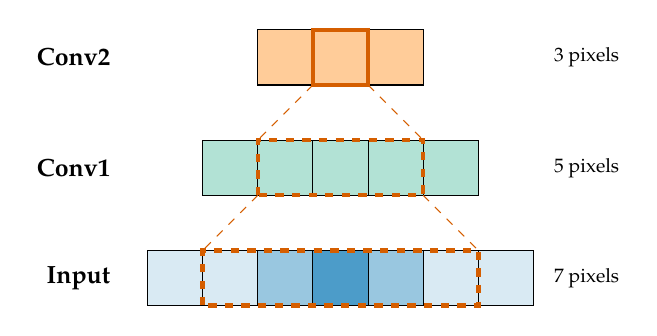
\begin{tikzpicture}[scale=0.7]
    % Layer 0: Input (7 pixels)
    \node[left, font=\small] at (-0.5, 0.5) {\textbf{Input}};
    \foreach \i/\c in {0/15, 1/15, 2/40, 3/70, 4/40, 5/15, 6/15} {
        \draw[fill=blue!\c, draw=black] (\i, 0) rectangle ++(1, 1);
    }
    \node[right, font=\scriptsize] at (7.2, 0.5) {7 pixels};

    % Layer 1: After Conv1 (5 pixels)
    \node[left, font=\small] at (-0.5, 2.5) {\textbf{Conv1}};
    \foreach \i in {1,2,3,4,5} {
        \draw[fill=green!30, draw=black] (\i, 2) rectangle ++(1, 1);
    }
    \node[right, font=\scriptsize] at (7.2, 2.5) {5 pixels};

    % Layer 2: After Conv2 (3 pixels)
    \node[left, font=\small] at (-0.5, 4.5) {\textbf{Conv2}};
    \foreach \i in {2,3,4} {
        \draw[fill=orange!40, draw=black] (\i, 4) rectangle ++(1, 1);
    }
    \node[right, font=\scriptsize] at (7.2, 4.5) {3 pixels};

    % Highlight target neuron at center of Conv2
    \draw[red, ultra thick] (3, 4) rectangle (4, 5);

    % It depends on 3 cells in Conv1 (cells 2, 3, 4)
    \draw[red, ultra thick, dashed] (2, 2) rectangle (5, 3);
    \draw[red, dashed] (3, 4) -- (2, 3);
    \draw[red, dashed] (4, 4) -- (5, 3);

    % Which depend on 5 cells in Input (cells 1, 2, 3, 4, 5)
    \draw[red, ultra thick, dashed] (1, 0) rectangle (6, 1);
    \draw[red, dashed] (2, 2) -- (1, 1);
    \draw[red, dashed] (5, 2) -- (6, 1);
\end{tikzpicture}
\end{center}

\vspace{4pt}
\textbf{Verify with the formula:}
\begin{itemize}
    \item Layer 1: $\text{RF}_1 = 1 + (3-1) \cdot 1 = 3$ \quad $\checkmark$ (red box at Conv1 spans 3 cells).
    \item Layer 2: $\text{RF}_2 = 3 + (3-1) \cdot 1 = 5$ \quad $\checkmark$ (red box at Input spans 5 cells).
\end{itemize}
\end{frame}

% ---- Visualizing the Jump ----
\begin{frame}
\frametitle{Visualizing the Jump After Pooling}

\textbf{Key idea:} after a pooling layer with stride 2, each pixel in the next layer corresponds to \textbf{2 input pixels}, not 1.

\vspace{6pt}
\begin{center}
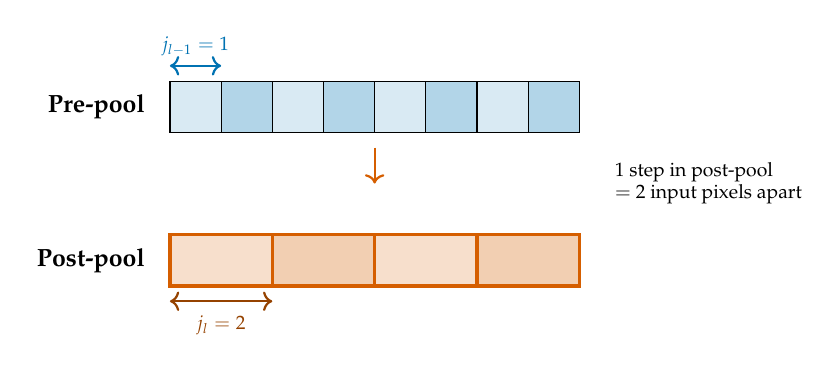
\begin{tikzpicture}[scale=0.65]
    % Pre-pool layer
    \node[left, font=\small] at (-0.3, 0.5) {\textbf{Pre-pool}};
    \foreach \i/\c in {0/blue!15, 1/blue!30, 2/blue!15, 3/blue!30, 4/blue!15, 5/blue!30, 6/blue!15, 7/blue!30} {
        \draw[fill=\c, draw=black] (\i, 0) rectangle ++(1, 1);
    }

    % Pool 2x2, stride 2
    \draw[->, thick, red] (4, -0.3) -- (4, -1);

    % Post-pool layer (4 pixels, each "sees" 2 pre-pool)
    \node[left, font=\small] at (-0.3, -2.5) {\textbf{Post-pool}};
    \foreach \i/\c in {0/red!20, 2/red!30, 4/red!20, 6/red!30} {
        \draw[fill=\c, draw=red, very thick] (\i, -3) rectangle ++(2, 1);
    }

    % Show jump
    \draw[<->, thick, blue] (0, 1.3) -- (1, 1.3);
    \node[above, font=\scriptsize, text=blue] at (0.5, 1.3) {$j_{l-1} = 1$};

    \draw[<->, thick, red!70!black] (0, -3.3) -- (2, -3.3);
    \node[below, font=\scriptsize, text=red!70!black] at (1, -3.4) {$j_l = 2$};

    % Now 1 step in post-pool = 2 input pixels
    \node[right, font=\scriptsize, align=left] at (8.5, -1) {1 step in post-pool\\$=$ 2 input pixels apart};
\end{tikzpicture}
\end{center}

\vspace{6pt}
\textbf{Consequence:} when the next $3 \times 3$ conv slides over the post-pool layer, those 3 ``adjacent'' positions are actually \textbf{6 input pixels apart}!

\vspace{4pt}
That's why the formula has $(F-1) \cdot j_{l-1}$ --- each kernel step covers $j_{l-1}$ input pixels.

\textcolor{red}{The jump factor $j$ explains the multiplier on receptive field growth.}
\end{frame}

% ---- With vs Without Pooling Comparison ----
\begin{frame}
\frametitle{With vs Without Pooling: RF Comparison}

Same network architecture, but compare RF growth \textbf{with} and \textbf{without} pooling:

\vspace{6pt}
\renewcommand{\arraystretch}{1.2}
\begin{center}
{\footnotesize
\begin{tabular}{c|ccccccc}
\toprule
\textbf{Layer} & 1 & 2 & 3 & 4 & 5 & 6 & 7 \\
\midrule
Operation (no pool) & Conv & Conv & Conv & Conv & Conv & Conv & Conv \\
RF (no pool) & 3 & 5 & 7 & 9 & 11 & 13 & \textcolor{blue}{\textbf{15}} \\
\midrule
Operation (with pool) & Conv & Conv & Pool & Conv & Conv & Pool & Conv \\
RF (with pool) & 3 & 5 & 6 & 10 & 14 & 16 & \textcolor{red}{\textbf{24}} \\
\bottomrule
\end{tabular}
}
\end{center}

\vspace{6pt}
\textbf{Without pooling:} RF grows \textbf{linearly}, $\text{RF}_l = 2l + 1$. Need many layers to ``see'' a large area.

\textbf{With pooling:} RF grows \textbf{multiplicatively}. Each pool doubles future increments.

\vspace{6pt}
\textbf{To cover a $32 \times 32$ image:}
\begin{itemize}
    \item Without pooling: need $L = 16$ conv layers ($\text{RF} = 33$).
    \item With pooling: need only $\sim 7$ layers (as shown).
\end{itemize}

\textcolor{red}{Pooling makes deep networks \textbf{practical}.}
\end{frame}

% ---- Receptive Field Visual Intuition ----
\begin{frame}
\frametitle{What Does Each Layer ``See''?}

The receptive field tells us \textbf{how much of the input image} a neuron at a given layer ``sees''.

\vspace{4pt}
\begin{center}
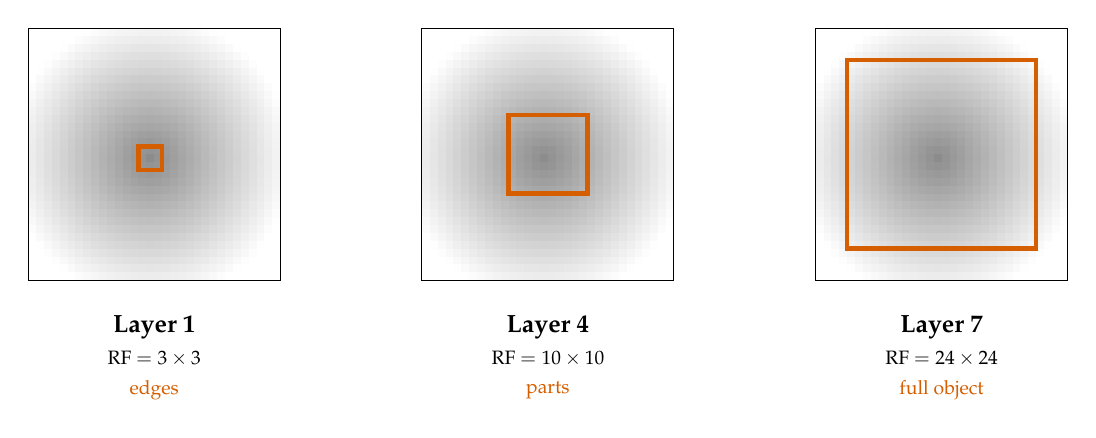
\begin{tikzpicture}
% Three 32x32 grids side by side, with simulated blob in the center
\foreach \shift/\rfsize/\rflo/\rfhi in {0/3/14/17, 5/10/11/21, 10/24/4/28} {
    \begin{scope}[xshift=\shift cm, scale=0.1]
        \foreach \i in {0,...,31} {
            \foreach \j in {0,...,31} {
                \pgfmathsetmacro{\dx}{\i-15}
                \pgfmathsetmacro{\dy}{\j-15}
                \pgfmathsetmacro{\d}{sqrt(\dx*\dx + \dy*\dy)}
                \pgfmathsetmacro{\b}{max(0, 90 - 5*\d)}
                \fill[gray!\b!white] (\i, \j) rectangle ++(1, 1);
            }
        }
        \draw[black, thin] (0, 0) rectangle (32, 32);
        \draw[red, ultra thick] (\rflo, \rflo) rectangle (\rfhi, \rfhi);
    \end{scope}
}

% Labels
\node[font=\small\bfseries] at (1.6, -0.6) {Layer 1};
\node[font=\scriptsize] at (1.6, -1.0) {RF $= 3 \times 3$};
\node[font=\scriptsize, text=red] at (1.6, -1.4) {edges};

\node[font=\small\bfseries] at (6.6, -0.6) {Layer 4};
\node[font=\scriptsize] at (6.6, -1.0) {RF $= 10 \times 10$};
\node[font=\scriptsize, text=red] at (6.6, -1.4) {parts};

\node[font=\small\bfseries] at (11.6, -0.6) {Layer 7};
\node[font=\scriptsize] at (11.6, -1.0) {RF $= 24 \times 24$};
\node[font=\scriptsize, text=red] at (11.6, -1.4) {full object};
\end{tikzpicture}
\end{center}

\vspace{4pt}
\textbf{Hierarchical features:} early layers detect \textbf{edges}, middle layers detect \textbf{parts} (an eye, a wheel), deep layers recognize \textbf{full objects/scenes}.

\textcolor{red}{Depth matters: each layer \textbf{composes} features from the previous one.}
\end{frame}


% ============================================================
\section{Pooling}
% ============================================================

\begin{transitionframe}
\begin{center}
{\Huge \textbf{Pooling}}
\end{center}
\end{transitionframe}

\begin{frame}
\frametitle{Pooling: Aggregation and Downsampling}

\textbf{Pooling} aggregates values in local regions of a feature map.

\vspace{6pt}
\begin{center}
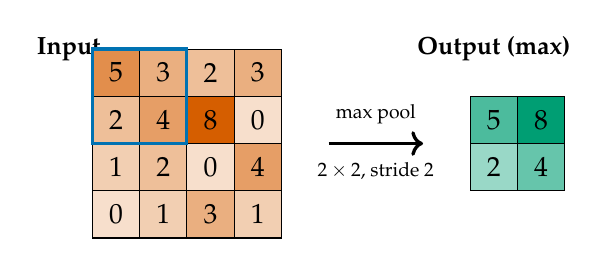
\begin{tikzpicture}[scale=0.6]
    % Input
    \node at (-0.5, 4) {\small \textbf{Input}};
    \foreach \i/\j/\v in {0/0/5, 1/0/3, 2/0/2, 3/0/3,
                          0/1/2, 1/1/4, 2/1/8, 3/1/0,
                          0/2/1, 1/2/2, 2/2/0, 3/2/4,
                          0/3/0, 1/3/1, 2/3/3, 3/3/1} {
        \pgfmathsetmacro{\col}{20 + 10*\v}
        \draw[fill=red!\col] (\i, 3-\j) rectangle ++(1, 1);
        \node at (\i+0.5, 3-\j+0.5) {\v};
    }
    \draw[blue, very thick] (0, 2) rectangle (2, 4);

    % Arrow
    \draw[->, very thick] (5, 2) -- (7, 2);
    \node[above, font=\scriptsize] at (6, 2.2) {max pool};
    \node[below, font=\scriptsize] at (6, 1.8) {$2 \times 2$, stride $2$};

    % Output (max pool)
    \node at (8.5, 4) {\small \textbf{Output (max)}};
    \foreach \i/\j/\v in {0/0/5, 1/0/8,
                          0/1/2, 1/1/4} {
        \pgfmathsetmacro{\col}{20 + 10*\v}
        \draw[fill=green!\col] (8+\i, 2-\j) rectangle ++(1, 1);
        \node at (8.5+\i, 2-\j+0.5) {\v};
    }
\end{tikzpicture}
\end{center}

\vspace{4pt}
\textbf{Two main types:}
\begin{itemize}
    \item \textbf{Max pooling:} take the maximum value in each window. Most common.
    \item \textbf{Average pooling:} take the average. Sometimes used in final layers.
\end{itemize}

\vspace{4pt}
\textbf{Why pool?}
(1) \textbf{Downsampling} (reduces computation and parameters);
(2) \textbf{Translation invariance} (small shifts don't change max).
\end{frame}

\begin{frame}
\frametitle{Pooling vs Strided Convolutions}

\textbf{Modern alternative:} use \textbf{strided convolutions} ($S = 2$) instead of pooling.

\vspace{4pt}
\renewcommand{\arraystretch}{1.3}
\begin{center}
{\small
\begin{tabular}{lll}
\toprule
& \textbf{Pooling} & \textbf{Strided Convolution} \\
\midrule
Operation & Max / Average (no params) & Learnable filter with $S=2$ \\
Parameters & 0 & $F \times F \times C_{in} \times C_{out}$ \\
Used in & LeNet, AlexNet, VGG & ResNet, modern architectures \\
\bottomrule
\end{tabular}
}
\end{center}

\vspace{4pt}
\textbf{Trend:} modern architectures prefer strided convs because the network \textbf{learns the optimal downsampling}.

\vspace{4pt}
\textbf{Pop quiz}: a $5\times 5\times 16$ input with 36 filters of $3\times 3$ (stride 1, no padding):
\begin{itemize}
    \item Each filter: $3 \times 3 \times 16$ (matches input channels).
    \item Output: \textcolor{red}{$3 \times 3 \times 36$}.
\end{itemize}
\end{frame}


% ============================================================
\section{Classic Architectures}
% ============================================================

\begin{transitionframe}
\begin{center}
{\Huge \textbf{Classic CNN Architectures}}
\end{center}
\end{transitionframe}

\begin{frame}
\frametitle{LeNet-5 (LeCun et al., 1998)}

\textbf{First successful CNN.} Designed for handwritten digit recognition (MNIST).

\vspace{6pt}
\begin{center}
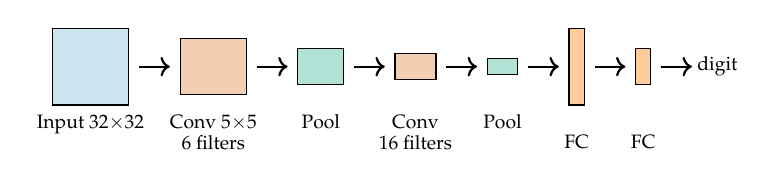
\begin{tikzpicture}[scale=0.65]
    \draw[fill=blue!20] (0, 0) rectangle (1.5, 1.5);
    \node[below] at (0.75, 0) {\scriptsize Input $32{\times}32$};

    \draw[->, thick] (1.7, 0.75) -- (2.3, 0.75);
    \draw[fill=red!30] (2.5, 0.2) rectangle (3.8, 1.3);
    \node[below] at (3.15, 0) {\scriptsize Conv $5{\times}5$};
    \node[below] at (3.15, -0.4) {\scriptsize 6 filters};

    \draw[->, thick] (4, 0.75) -- (4.6, 0.75);
    \draw[fill=green!30] (4.8, 0.4) rectangle (5.7, 1.1);
    \node[below] at (5.25, 0) {\scriptsize Pool};

    \draw[->, thick] (5.9, 0.75) -- (6.5, 0.75);
    \draw[fill=red!30] (6.7, 0.5) rectangle (7.5, 1);
    \node[below] at (7.1, 0) {\scriptsize Conv};
    \node[below] at (7.1, -0.4) {\scriptsize 16 filters};

    \draw[->, thick] (7.7, 0.75) -- (8.3, 0.75);
    \draw[fill=green!30] (8.5, 0.6) rectangle (9.1, 0.9);
    \node[below] at (8.8, 0) {\scriptsize Pool};

    \draw[->, thick] (9.3, 0.75) -- (9.9, 0.75);
    \draw[fill=orange!40] (10.1, 0) rectangle (10.4, 1.5);
    \node[below] at (10.25, -0.4) {\scriptsize FC};

    \draw[->, thick] (10.6, 0.75) -- (11.2, 0.75);
    \draw[fill=orange!40] (11.4, 0.4) rectangle (11.7, 1.1);
    \node[below] at (11.55, -0.4) {\scriptsize FC};

    \draw[->, thick] (11.9, 0.75) -- (12.5, 0.75);
    \node at (13, 0.75) {\scriptsize digit};
\end{tikzpicture}
\end{center}

\vspace{8pt}
\textbf{Key innovations:}
\begin{itemize}
    \item Conv $\to$ Pool $\to$ Conv $\to$ Pool $\to$ FC pattern (still standard today).
    \item Tanh activation, average pooling.
    \item About \textbf{60,000 parameters}.
\end{itemize}

\vspace{4pt}
\textcolor{red}{Limitation:} too small for natural images. Required compute didn't exist for larger versions.
\end{frame}

\begin{frame}
\frametitle{AlexNet (Krizhevsky et al., 2012)}

\textbf{The ImageNet revolution.} Won ILSVRC 2012 by a huge margin (top-5 error: 16\% vs 26\%).

\vspace{6pt}
\textbf{Architecture:} 5 conv layers + 3 FC layers, $\sim$ \textbf{60 million parameters}.

\vspace{6pt}
\textcolor{blue}{\textbf{Key innovations:}}
\begin{itemize}
    \item \textbf{ReLU} activations (faster training than tanh/sigmoid).
    \item \textbf{Dropout} for regularization.
    \item Trained on \textbf{2 GPUs} (model parallelism due to memory limits).
    \item \textbf{Data augmentation} (random crops, color jittering).
    \item Trained on \textbf{ImageNet} (1.2M images, 1000 classes).
\end{itemize}

\vspace{8pt}
\begin{center}
\textcolor{red}{\textbf{This paper kickstarted the modern deep learning era.}}
\end{center}
\end{frame}

\begin{frame}
\frametitle{VGG (Simonyan \& Zisserman, 2014)}

\textbf{Idea:} use \textbf{small} $3 \times 3$ filters but stack \textbf{many} layers.

\vspace{6pt}
\textbf{VGG-16 architecture:} 13 conv layers + 3 FC layers, \textbf{138 million parameters}.

\vspace{8pt}
\textbf{Why $3 \times 3$ filters?} Stacking two $3 \times 3$ convs has the same receptive field as one $5 \times 5$ conv, but with:
\begin{itemize}
    \item \textbf{Fewer parameters:} $2 \cdot 3^2 = 18$ vs $5^2 = 25$.
    \item \textbf{More non-linearities} (two ReLUs vs one).
    \item \textbf{Better expressivity} for the same receptive field.
\end{itemize}

\vspace{8pt}
\begin{tikzpicture}
\node [mybox] (box){%
    \begin{minipage}{0.93\textwidth}
    \vspace{-4pt}
    \textbf{The VGG insight:} \textbf{depth} matters more than filter size. Use uniform $3 \times 3$ convolutions and let depth do the work.
    \end{minipage}
};
\node[fancytitle, right=10pt] at (box.north west) {Key Insight};
\end{tikzpicture}
\end{frame}

\begin{frame}
\frametitle{ResNet (He et al., 2015)}

\textbf{The degradation problem:} as networks get deeper (50+ layers), training loss \textbf{increases}, not just test loss.

\vspace{6pt}
\textbf{Solution:} \textbf{residual / skip connections}.

\begin{center}
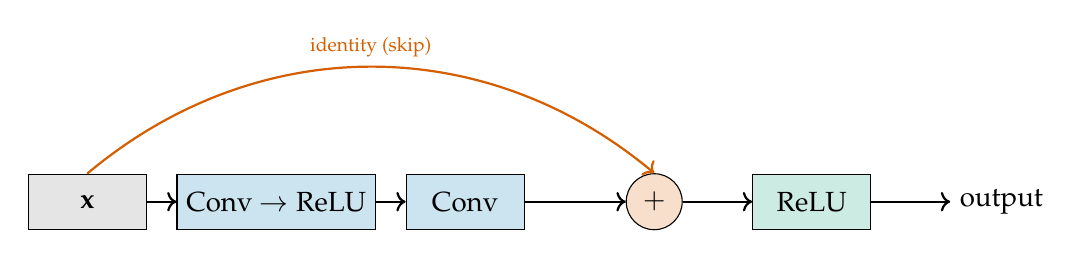
\begin{tikzpicture}[scale=0.8]
    \node[draw, fill=gray!20, minimum width=1.5cm, minimum height=0.7cm] (x) at (0, 0) {$\vx$};
    \node[draw, fill=blue!20, minimum width=1.5cm, minimum height=0.7cm] (l1) at (3, 0) {Conv $\to$ ReLU};
    \node[draw, fill=blue!20, minimum width=1.5cm, minimum height=0.7cm] (l2) at (6, 0) {Conv};
    \node[draw, circle, fill=red!20, minimum size=0.7cm] (plus) at (9, 0) {$+$};
    \node[draw, fill=green!20, minimum width=1.5cm, minimum height=0.7cm] (relu) at (11.5, 0) {ReLU};
    \node[right=1cm of relu] (out) {output};

    \draw[->, thick] (x) -- (l1);
    \draw[->, thick] (l1) -- (l2);
    \draw[->, thick] (l2) -- (plus);
    \draw[->, thick] (plus) -- (relu);
    \draw[->, thick] (relu) -- (out);

    % Skip connection
    \draw[->, thick, red] (x.north) to[bend left=40] node[above, font=\scriptsize, text=red] {identity (skip)} (plus.north);
\end{tikzpicture}
\end{center}

\vspace{6pt}
\textbf{Mathematical formulation:} \quad $\vh^{(l+1)} = \mathcal{F}(\vh^{(l)}; \vW^{(l)}) + \vh^{(l)}$

\vspace{4pt}
\textbf{Why this works:}
\begin{itemize}
    \item Gradient flow: $\nabla \vh^{(l)}$ has a direct path back via the identity (no vanishing gradient).
    \item If the optimal layer is identity, the network can easily learn $\mathcal{F} \approx 0$.
    \item Allows training networks with \textbf{152, 1000+ layers}.
\end{itemize}
\end{frame}

\begin{frame}
\frametitle{Architecture Evolution: A Visual Summary}

\renewcommand{\arraystretch}{1.4}
\begin{center}
{\small
\begin{tabular}{lcccl}
\toprule
\textbf{Architecture} & \textbf{Year} & \textbf{Layers} & \textbf{Params} & \textbf{Key idea} \\
\midrule
LeNet-5 & 1998 & 7 & 60K & First successful CNN \\
AlexNet & 2012 & 8 & 60M & ReLU + Dropout + GPU \\
VGG-16 & 2014 & 16 & 138M & Uniform $3\times3$ filters \\
GoogLeNet & 2014 & 22 & 6.8M & Inception modules \\
ResNet-152 & 2015 & 152 & 60M & \textcolor{red}{Skip connections} \\
DenseNet & 2017 & 121+ & 8M & Dense skip connections \\
EfficientNet & 2019 & varies & 5--66M & Compound scaling \\
\bottomrule
\end{tabular}
}
\end{center}

\vspace{4pt}
\textbf{General trends:} deeper networks $\cdot$ smaller filters ($3\times 3$ standard) $\cdot$ skip connections $\cdot$ better parameter efficiency.
\end{frame}


% ============================================================
\section{Applications in Economics}
% ============================================================

\begin{transitionframe}
\begin{center}
{\Huge \textbf{Applications in Economics}}
\end{center}
\end{transitionframe}

\begin{frame}
\frametitle{Predicting Poverty from Satellite Imagery}

\begin{tikzpicture}
\node [mybox] (box){%
    \begin{minipage}{0.93\textwidth}
    \vspace{-4pt}
    \textbf{Jean, Burke, Xie, Davis, Lobell, Ermon (2016).} Combining Satellite Imagery and Machine Learning to Predict Poverty. \textit{Science}, 353(6301), 790--794.
    \end{minipage}
};
\node[fancytitle, right=10pt] at (box.north west) {Landmark Paper};
\end{tikzpicture}

\vspace{4pt}
\textbf{Problem:} household survey data is scarce in many African countries. Can we predict consumption from satellite imagery?

\vspace{4pt}
\textbf{Pipeline:}
\begin{enumerate}
    \item Take a \textbf{pretrained CNN} (VGG on ImageNet).
    \item Fine-tune on satellite imagery to predict \textbf{nightlight intensity} (proxy for activity).
    \item Use learned features to predict \textbf{household consumption} from daytime images.
\end{enumerate}

\vspace{4pt}
\textbf{Result:} explained up to \textbf{75\% of variation} in local economic outcomes across 5 African countries.

\textcolor{red}{This is \textbf{transfer learning} --- covered more in Lecture 9.}
\end{frame}

\begin{frame}
\frametitle{Other Economic Applications of CNNs}

\textbf{Land use and agricultural monitoring:}
\begin{itemize}
    \item \textbf{Crop yield prediction} from satellite imagery (You, Li, Low, Lobell, Ermon, 2017).
    \item \textbf{Deforestation tracking} for environmental economics.
    \item \textbf{Land cover classification} (USDA, ESA).
\end{itemize}

\vspace{6pt}
\textbf{Real estate and urban economics:}
\begin{itemize}
    \item \textbf{Property valuation} from street view images (Naik et al., 2017).
    \item \textbf{Neighborhood characteristics} from urban imagery (Glaeser, Kominers et al., 2018).
    \item \textbf{Gentrification detection} from time-series imagery.
\end{itemize}

\vspace{6pt}
\textbf{Development economics:}
\begin{itemize}
    \item \textbf{Wealth indices} from satellite + survey data (Yeh et al., 2020).
    \item \textbf{Health outcomes} from environmental imagery.
    \item \textbf{Conflict and disaster damage} from before/after imagery.
\end{itemize}
\end{frame}



% ============================================================
\section{PyTorch Implementation}
% ============================================================

\begin{transitionframe}
\begin{center}
{\Huge \textbf{PyTorch Implementation}}
\end{center}
\end{transitionframe}

\begin{frame}[fragile]
\frametitle{Building a Simple CNN in PyTorch}

\begin{lstlisting}
import torch
import torch.nn as nn

class SimpleCNN(nn.Module):
    def __init__(self, num_classes=10):
        super().__init__()
        # Input: 3 x 32 x 32 (CIFAR-10)
        self.conv1 = nn.Conv2d(3, 32, kernel_size=3, padding=1)
        self.conv2 = nn.Conv2d(32, 64, kernel_size=3, padding=1)
        self.pool  = nn.MaxPool2d(2, 2)
        self.fc1   = nn.Linear(64 * 8 * 8, 128)
        self.fc2   = nn.Linear(128, num_classes)

    def forward(self, x):
        x = self.pool(torch.relu(self.conv1(x)))   # 32 x 16 x 16
        x = self.pool(torch.relu(self.conv2(x)))   # 64 x 8 x 8
        x = x.flatten(1)                           # 64*8*8
        x = torch.relu(self.fc1(x))
        return self.fc2(x)
\end{lstlisting}
\end{frame}

\begin{frame}[fragile]
\frametitle{Using a Pretrained ResNet}

\textbf{Transfer learning:} use a network pretrained on ImageNet, fine-tune for your task.

\vspace{4pt}
\begin{lstlisting}
import torch
import torchvision.models as models
import torch.nn as nn

# Load pretrained ResNet-50
model = models.resnet50(weights='IMAGENET1K_V2')

# Freeze all parameters
for param in model.parameters():
    param.requires_grad = False

# Replace the final FC layer for our task (e.g., 5 classes)
model.fc = nn.Linear(model.fc.in_features, 5)

# Only the new FC layer will be trained
optimizer = torch.optim.Adam(model.fc.parameters(), lr=1e-3)
\end{lstlisting}

\vspace{4pt}
\textbf{This is the technique used in Jean et al.\ (2016).}
\end{frame}


% ============================================================
\section{Summary and Next Steps}
% ============================================================

\begin{transitionframe}
\begin{center}
{\Huge \textbf{Summary \& Next Steps}}
\end{center}
\end{transitionframe}

\begin{frame}
\frametitle{Summary}

\begin{enumerate}
    \item \textbf{Inductive biases for images:} locality + translation invariance.

    \item \textbf{Convolution:} slide a small kernel across the input, compute dot products. Output size: $\lfloor (W + 2P - F)/S \rfloor + 1$.

    \item \textbf{Multi-channel convolutions:} kernel has the same number of channels as input; multiple kernels produce multiple output feature maps.

    \item \textbf{Pooling}: aggregates feature values for downsampling and invariance.

    \item \textbf{Classic architectures:} LeNet $\to$ AlexNet $\to$ VGG $\to$ ResNet (skip connections enable very deep networks).

    \item \textbf{Economic applications:} satellite imagery for poverty prediction, land use classification, real estate, etc.

    \item \textbf{Transfer learning:} fine-tune ImageNet-pretrained models for new tasks.
\end{enumerate}
\end{frame}

\begin{frame}
\frametitle{Next Lecture: Word Embeddings \& RNNs}

\textbf{Lecture 5} (Monday, April 27):
\begin{itemize}
    \item Word2Vec: representing words as vectors.
    \item Skip-gram and CBOW.
    \item Recurrent Neural Networks (RNNs).
    \item LSTM and GRU.
    \item Applications to text and time series.
\end{itemize}

\vspace{6pt}
\textbf{Recommended reading:}
\begin{itemize}
    \item Goodfellow et al., \textit{Deep Learning}, Chapter 9 (CNNs).
    \item He et al.\ (2015), \textit{Deep Residual Learning for Image Recognition}.
    \item Jean et al.\ (2016), \textit{Combining Satellite Imagery and ML to Predict Poverty}.
\end{itemize}

\vspace{6pt}
\textbf{Homework 2} will be released after Lecture 5 (covers CNNs).

\vspace{4pt}
\begin{center}
\Large \textcolor{blue}{\textbf{Questions?}}
\end{center}
\end{frame}

\begin{frame}
\frametitle{References}

\footnotesize
\begin{itemize}
    \item LeCun, Y., Bottou, L., Bengio, Y., \& Haffner, P. (1998). Gradient-based learning applied to document recognition. \textit{Proceedings of the IEEE}.
    \item Krizhevsky, A., Sutskever, I., \& Hinton, G. E. (2012). ImageNet classification with deep convolutional neural networks. \textit{NeurIPS}.
    \item Simonyan, K., \& Zisserman, A. (2014). Very deep convolutional networks for large-scale image recognition (VGG). \textit{ICLR}.
    \item He, K., Zhang, X., Ren, S., \& Sun, J. (2015). Deep residual learning for image recognition (ResNet). \textit{CVPR}.
    \item Jean, N., Burke, M., Xie, M., Davis, W. M., Lobell, D. B., \& Ermon, S. (2016). Combining satellite imagery and machine learning to predict poverty. \textit{Science}, 353(6301).
    \item You, J., Li, X., Low, M., Lobell, D., \& Ermon, S. (2017). Deep Gaussian process for crop yield prediction based on remote sensing data. \textit{AAAI}.
    \item Yeh, C. et al. (2020). Using publicly available satellite imagery and deep learning to understand economic well-being in Africa. \textit{Nature Communications}.
\end{itemize}
\end{frame}


\end{document}
